\documentclass[12pt,a4paper]{article}

\usepackage[margin=2.54cm]{geometry}
\usepackage{iftex}
\ifPDFTeX
  \usepackage[T1]{fontenc}
  \usepackage{newtxtext,newtxmath}
\else
  \usepackage{fontspec}
  \setmainfont{Times New Roman}
  \usepackage{unicode-math}
  \setmathfont{TeX Gyre Termes Math}
\fi
\usepackage{amsmath}
\usepackage{booktabs}
\usepackage{graphicx}
\graphicspath{{../outputs/figures/}{outputs/figures/}}
\usepackage{float}
\usepackage{caption}
\usepackage{pdflscape}
\usepackage[round,authoryear]{natbib}
\setcitestyle{aysep={,},yysep={;}}
\usepackage{xurl}
\usepackage[hidelinks]{hyperref}
\usepackage{setspace}

\onehalfspacing
\setlength{\parindent}{0pt}
\setlength{\parskip}{\baselineskip}
\setlength{\emergencystretch}{3em}
\pagestyle{empty}
\captionsetup{font=small,labelfont=bf,justification=centering}

\newcommand{\PaperTitle}{Time-Varying Volatility Connectedness among ASEAN Equity Markets:\\
Evidence from Global Geopolitical and Macroeconomic Shocks}

\begin{document}

\begin{center}
{\Large\bfseries \PaperTitle\par}
\end{center}

\begin{abstract}
This study examines the magnitude, direction, and evolution of volatility transmission among the equity markets of Indonesia, Malaysia, the Philippines, Singapore, Thailand, and Vietnam from January 2010 to July 2026. Using range-based volatility and a generalized forecast-error variance-decomposition framework, the study estimates total, directional, pairwise, and net connectedness. Full-sample volatility connectedness is approximately 17.15\%, while the mean 250-day rolling index is 20.04\%. Thailand and Indonesia are net transmitters in the baseline model, whereas Vietnam is a modest net receiver and exhibits the largest own-market variance share. Moving-block bootstrap comparisons identify significant shock-associated increases in six of eight prespecified episodes, with the largest increase occurring during the COVID-19 pandemic. Monthly regressions with heteroskedasticity- and autocorrelation-consistent inference show that the VIX and oil-price changes are positively associated with regional connectedness, while geopolitical risk is negatively associated with it. Vietnam's directional role is sensitive to the volatility proxy and currency denomination, cautioning against a fixed classification of the market as a transmitter or receiver. The findings demonstrate that ASEAN systemic risk is strongly time varying and that diversification benefits can weaken precisely when global uncertainty is elevated.

\textbf{Keywords:} ASEAN equity markets; volatility spillovers; financial connectedness; systemic risk; geopolitical risk; Vietnam

\textbf{JEL classification:} C32; F36; G11; G15
\end{abstract}

\section{Introduction}

The increasing integration of ASEAN economies has expanded opportunities for cross-border investment, financing, and risk sharing. At the same time, closer financial links can provide channels through which shocks originating in one market are transmitted to others. This tension is especially important in Southeast Asia, where equity markets differ substantially in size, liquidity, foreign-investor participation, exchange-rate exposure, and institutional development. A disturbance that is absorbed locally in one market may therefore produce persistent regional effects in another.

The period since 2010 provides a particularly useful setting in which to examine these linkages. ASEAN markets have experienced the consequences of the European sovereign-debt crisis, the taper tantrum, trade tensions between the United States and China, the COVID-19 pandemic, Russia's invasion of Ukraine, rapid monetary tightening in advanced economies, and renewed geopolitical instability. These episodes affected global risk appetite, funding conditions, commodity prices, and international capital flows. However, the existence of common global shocks does not imply that all ASEAN markets transmit or absorb risk in the same way. Identifying the direction of transmission is therefore as important as measuring its overall magnitude.

Existing evidence documents important linkages between Asian equity markets and shows that market openness is related to exposure to external volatility \citep{Chow2017}. Research focused on ASEAN also finds significant volatility transmission from the United States \citep{VoTran2020}, while evidence for Vietnam indicates meaningful linkages with advanced markets \citep{VoEllis2018}. Recent studies have moved closer to the present setting. \citet{SethapramoteEtAl2023} examine dynamic connectedness between ASEAN and global equity markets during COVID-19, while \citet{AlAnshari2025} studies the evolution of an ASEAN-6 network, including Vietnam, using correlation- and graph-based methods. Work on categorical policy uncertainty further demonstrates that the magnitude and direction of ASEAN connectedness depend on the source and timing of uncertainty \citep{HoqueEtAl2026}. Consequently, the remaining gap is not the absence of ASEAN network evidence. Rather, three issues remain unresolved. First, Vietnam's directional role within an internally focused ASEAN volatility network remains sensitive to how volatility and market integration are measured. Second, average full-sample estimates can conceal changes in the identity of net shock transmitters and receivers across multiple global episodes. Third, high comovement during turbulent periods should not automatically be described as contagion. As emphasized by \citet{ForbesRigobon2002}, contagion requires an increase in cross-market linkages following a shock; otherwise, the evidence may reflect continuing interdependence.

This paper addresses these issues by estimating the dynamic volatility connectedness of six ASEAN equity markets: Indonesia, Malaysia, the Philippines, Singapore, Thailand, and Vietnam. The empirical framework is based on generalized forecast-error variance decompositions from a vector autoregression (VAR). It measures the share of each market's forecast-error variance attributable to shocks from every other market, without making the results dependent on the ordering of variables \citep{PesaranShin1998,DieboldYilmaz2012}. Rolling-window estimation then reveals changes in regional connectedness and in each market's systemic role over time.

The paper asks four questions. First, how strongly are volatility shocks transmitted among ASEAN equity markets? Second, which markets are net transmitters and which are net receivers of volatility? Third, does Vietnam's role in the network change across tranquil and turbulent periods? Fourth, do geopolitical and macroeconomic shocks produce statistically and economically meaningful increases in regional connectedness?

The study makes three contributions relative to this literature. First, it estimates an internally focused ASEAN-6 directional volatility network over 2010--2026 and evaluates Vietnam's role using range-based and return-based volatility measures, local- and US-dollar returns, and daily and weekly frequencies. Second, it tracks changes in both aggregate connectedness and transmitter--receiver positions across eight global shock episodes rather than concentrating on COVID-19 alone. Third, it distinguishes persistent interdependence from shock-associated increases using fixed event definitions and dependence-preserving bootstrap inference. These features complement the global-market emphasis of \citet{SethapramoteEtAl2023} and the correlation- and graph-based network analysis of \citet{AlAnshari2025}.

The remainder of the paper is organized as follows. Section~\ref{sec:literature} reviews the related literature and develops the hypotheses. Section~\ref{sec:data} describes the data and construction of volatility measures. Section~\ref{sec:method} presents the connectedness framework and the tests for shock-related changes. Section~\ref{sec:results} sets out the empirical analysis. Section~\ref{sec:robustness} describes robustness tests, and Section~\ref{sec:conclusion} concludes.

\section{Related Literature and Hypotheses}
\label{sec:literature}

\subsection{Financial integration, spillovers, and contagion}

International financial integration can improve risk sharing and price discovery, but it can also accelerate the transmission of adverse information. Spillovers arise when innovations in one market explain subsequent returns or volatility in another. When such connections are stable features of an integrated system, they represent interdependence. In contrast, \citet{ForbesRigobon2002} define contagion in terms of a significant increase in cross-market linkages after a shock. This distinction is important because correlations often rise mechanically when volatility increases. The present study therefore uses ``connectedness'' and ``spillover'' for the general transmission of shocks and uses ``contagion'' only when the empirical analysis supports a discrete or statistically significant increase during a shock period.

ASEAN markets are likely to be linked through several channels. Common global investors can rebalance portfolios across the region; trade linkages can transmit changes in expected cash flows; exchange-rate and commodity-price movements can alter firm values; and global risk aversion can simultaneously tighten financing conditions. These mechanisms imply that regional volatility should increase when a global disturbance changes investors' risk-bearing capacity or information set.

\textbf{H1:} Total volatility connectedness among ASEAN equity markets increases during periods of elevated global geopolitical or macroeconomic stress.

\subsection{Directional and time-varying transmission}

Aggregate measures alone cannot identify the source of risk. A market can receive substantial volatility from the system while contributing little to other markets, or it can act as a regional transmission hub. Differences in capitalization, liquidity, openness, and information processing suggest that directional effects will be heterogeneous. Moreover, these roles need not be constant. A domestic policy event may temporarily turn a usual receiver into a transmitter, while a global shock may strengthen the influence of the most internationally integrated market.

The connectedness approach of \citet{DieboldYilmaz2012} is well suited to this question because it separates shocks transmitted \emph{to} a market from those transmitted \emph{from} it. Its network interpretation also permits each market to be represented as a node joined by weighted, directed edges \citep{DieboldYilmaz2014}.

Two recent ASEAN studies provide especially close benchmarks. \citet{SethapramoteEtAl2023} report that spillovers from global equity markets to ASEAN increased during COVID-19 and that the contribution of intraregional ASEAN spillovers also became more important. Using all six markets examined here, \citet{AlAnshari2025} documents crisis-related changes in ASEAN-6 correlation and network structure between 2011 and 2024. The present study differs by modeling volatility rather than return-network similarity, deriving directional shares from generalized forecast-error variance decompositions, examining several distinct global episodes, and formally testing shock-window differences.

\textbf{H2:} The magnitude and direction of volatility transmission are heterogeneous across ASEAN markets and vary over time.

Vietnam is a particularly informative case. Its equity market has become more integrated with international markets, but differences in market depth, investor composition, and institutional structure may affect how it absorbs external information. Rather than assuming a fixed role for Vietnam, the analysis tests whether it is generally a net receiver and identifies periods in which that position changes.

\textbf{H3:} Vietnam is, on average, a net receiver of volatility shocks within the ASEAN network, but its net connectedness changes across market regimes.

\subsection{Global uncertainty and regional connectedness}

Geopolitical events and macroeconomic policy shifts can affect ASEAN equities through global risk aversion, interest-rate expectations, exchange rates, trade, and commodity markets. Prior studies find meaningful connections between Asian equity volatility and external shocks \citep{Chow2017,VoTran2020}. These effects may be nonlinear: uncertainty can have modest consequences in normal conditions but large effects when market liquidity is limited or investors deleverage simultaneously.

\textbf{H4:} Higher global uncertainty is associated with stronger ASEAN volatility connectedness after controlling for general financial-market conditions.

\section{Data and Variable Construction}
\label{sec:data}

\subsection{Equity-market data}

The sample contains the principal broad equity indices for Indonesia, Malaysia, the Philippines, Singapore, Thailand, and Vietnam. Daily open, high, low, and closing index levels were collected from Yahoo Finance, with the VN-Index supplemented using VNStock. The raw sample runs from January 4, 2010 to July 17, 2026. Intersecting the six national trading calendars produces 3,366 common return observations. After requiring valid high and low prices, the baseline Parkinson-volatility panel contains 3,343 observations. Table~\ref{tab:markets} records the market series.

\begin{table}[H]
\centering
\caption{Equity-market series}
\label{tab:markets}
\begin{tabular}{llll}
\toprule
Country & Index & Vendor symbol & Currency \\
\midrule
Indonesia & Jakarta Composite Index & JKSE & IDR \\
Malaysia & FTSE Bursa Malaysia KLCI & KLSE & MYR \\
Philippines & PSE Composite Index & PSEI & PHP \\
Singapore & Straits Times Index & STI & SGD \\
Thailand & Stock Exchange of Thailand Index & SET & THB \\
Vietnam & VN-Index & VNINDEX & VND \\
\bottomrule
\end{tabular}
\begin{minipage}{0.92\textwidth}
\footnotesize\textit{Note:} Vendor symbols can vary across data services. The empirical files retain the original source, local currency, and raw trading date for every observation.
\end{minipage}
\end{table}

Continuously compounded daily returns for market $i$ are calculated as
\begin{equation}
 r_{i,t}=100\left[\ln(P_{i,t})-\ln(P_{i,t-1})\right],
 \label{eq:return}
\end{equation}
where $P_{i,t}$ is the closing index level. The baseline volatility proxy is the range-based estimator of \citet{Parkinson1980}:
\begin{equation}
 v_{i,t}=\frac{1}{4\ln(2)}\left[\ln\left(\frac{H_{i,t}}{L_{i,t}}\right)\right]^2,
 \label{eq:parkinson}
\end{equation}
where $H_{i,t}$ and $L_{i,t}$ denote the daily high and low. The VAR is estimated using $\ln(v_{i,t}+\epsilon)$, where $\epsilon$ is a small positive constant. Log squared returns and log absolute returns are used as alternative volatility proxies. Because national exchanges observe different holidays, the baseline panel retains only dates common to all six markets; prices are never carried forward and treated as new information. Local-currency measures form the baseline, while US-dollar return volatility and weekly observations provide robustness tests. Weekly high and low prices are respectively the maximum and minimum within each ISO week, and each week is assigned a common Friday date.

\subsection{Shock and uncertainty variables}

The dynamic analysis combines prespecified event windows with continuous global indicators. Monthly average VIX and geopolitical-risk (GPR) indices measure financial and geopolitical uncertainty. Brent crude oil prices, a broad US-dollar index, the S\&P 500, and the two-year US Treasury yield capture commodity, currency, equity, and monetary-policy conditions. VIX, Brent, Treasury-yield, dollar, and S\&P 500 observations are obtained through the Federal Reserve Economic Data service; the GPR index is from \citet{CaldaraIacoviello2022}. VIX and GPR enter as monthly averages. Oil, dollar, and S\&P 500 variables are end-of-month log changes in percent, while the Treasury yield is an end-of-month change in percentage points.

Eight event windows were fixed before the final results were interpreted. Their start dates are anchored to contemporaneous institutional records: the intensification of euro-area sovereign stress from mid-2011 \citep{ECB2012FSR}; Ben Bernanke's May 22, 2013 congressional testimony, which initiated the taper-tantrum repricing \citep{Bernanke2013}; the mid-2015 plunge in Chinese equities \citep{BIS2015China}; the March 22, 2018 announcement of US trade action against China \citep{USTR2018}; the World Health Organization's January 30, 2020 declaration of a Public Health Emergency of International Concern \citep{WHO2020}; Russia's February 24, 2022 invasion of Ukraine \citep{UNGA2022}; the Federal Reserve's sequence of 75-basis-point rate increases beginning in June 2022 \citep{FederalReserve2022}; and the March 10, 2023 closure of Silicon Valley Bank \citep{FederalReserve2023SVB}. End dates were set to capture the initial or sustained market-adjustment phase while preventing overlap between the two 2022 episodes. Table~\ref{tab:event-definitions} reports the exact analysis windows and preceding benchmarks used in the replication files.

\begin{table}[H]
\centering
\caption{Prespecified event and benchmark windows}
\label{tab:event-definitions}
\resizebox{\textwidth}{!}{%
\begin{tabular}{llll}
\toprule
Episode & Event window & Preceding benchmark & Date source \\
\midrule
European debt crisis & Jul. 1, 2011--Jun. 30, 2012 & Mar. 30--Jun. 30, 2011 & \citet{ECB2012FSR} \\
Taper tantrum & May 22--Sep. 30, 2013 & Jan. 2--May 21, 2013 & \citet{Bernanke2013} \\
China market crash & Jun. 12, 2015--Feb. 29, 2016 & Dec. 1, 2014--Jun. 11, 2015 & \citet{BIS2015China} \\
US--China trade war & Mar. 22--Dec. 31, 2018 & Sep. 1, 2017--Mar. 21, 2018 & \citet{USTR2018} \\
COVID-19 pandemic & Jan. 30--Jun. 30, 2020 & Jul. 1, 2019--Jan. 29, 2020 & \citet{WHO2020} \\
Russia--Ukraine war & Feb. 24--May 31, 2022 & Sep. 1, 2021--Feb. 23, 2022 & \citet{UNGA2022} \\
Global monetary tightening & Jun. 1--Dec. 31, 2022 & Sep. 1, 2021--Feb. 23, 2022 & \citet{FederalReserve2022} \\
US banking crisis & Mar. 10--May 31, 2023 & Dec. 1, 2022--Mar. 9, 2023 & \citet{FederalReserve2023SVB} \\
\bottomrule
\end{tabular}}
\begin{minipage}{0.94\textwidth}
\small\textit{Note:} Event definitions match \texttt{../deliverables/event\_windows.csv}. The shared pre-event benchmark for the two 2022 episodes avoids contamination by overlapping shock periods.
\end{minipage}
\end{table}

Each event is compared with its preceding benchmark, and inference uses moving-block bootstrap intervals with feasible block lengths of 10 and 20 trading days.

\begin{table}[H]
\centering
\caption{Variables, transformations, and sample coverage}
\label{tab:variables}
\begin{tabular}{p{0.19\textwidth}p{0.37\textwidth}p{0.25\textwidth}}
\toprule
Variable & Transformation & Source/frequency \\
\midrule
ASEAN volatility & $\ln\{[4\ln(2)]^{-1}[\ln(H/L)]^2+\epsilon\}$ & Yahoo Finance and VNStock; daily \\
Squared-return volatility & $\ln(r_{i,t}^{2}+\epsilon)$ & Constructed; daily and weekly \\
Absolute-return volatility & $\ln(|r_{i,t}|+\epsilon)$ & Constructed; daily and weekly \\
VIX & Monthly average of daily level & FRED; monthly \\
GPR & Monthly average of daily index & Caldara--Iacoviello; monthly \\
Oil, dollar, S\&P 500 & $100\Delta\ln(x_t)$ using month-end levels & FRED; monthly \\
US two-year yield & Month-end first difference, percentage points & FRED; monthly \\
\bottomrule
\end{tabular}
\begin{minipage}{0.86\textwidth}
\footnotesize\textit{Note:} The common daily return panel contains 3,366 observations from January 4, 2010 to July 17, 2026; the baseline volatility panel contains 3,343 observations. The rolling analysis produces 3,094 estimates with a 250-observation window.
\end{minipage}
\end{table}

\section{Methodology}
\label{sec:method}

\subsection{Generalized VAR connectedness}

Let $x_t=(v_{1,t},\ldots,v_{N,t})'$ denote the vector of volatility measures for the $N=6$ markets. Consider a covariance-stationary VAR($p$):
\begin{equation}
 x_t=\sum_{k=1}^{p}\Phi_k x_{t-k}+\varepsilon_t,
 \qquad \varepsilon_t\sim(0,\Sigma),
 \label{eq:var}
\end{equation}
where the lag length $p$ is selected using a prespecified information criterion and residual diagnostics. The moving-average representation is
\begin{equation}
 x_t=\sum_{h=0}^{\infty}A_h\varepsilon_{t-h},
 \label{eq:ma}
\end{equation}
with $A_0=I$ and recursively defined coefficient matrices $A_h$.

Following \citet{PesaranShin1998} and \citet{DieboldYilmaz2012}, the generalized $H$-step-ahead forecast-error variance contribution of shocks in market $j$ to the forecast-error variance of market $i$ is
\begin{equation}
 \theta_{ij}^{g}(H)=
 \frac{\sigma_{jj}^{-1}\sum_{h=0}^{H-1}
 \left(e_i'A_h\Sigma e_j\right)^2}
 {\sum_{h=0}^{H-1}e_i'A_h\Sigma A_h'e_i},
 \label{eq:gfevd}
\end{equation}
where $e_i$ is a selection vector with one in position $i$ and zeros elsewhere, and $\sigma_{jj}$ is the $j$th diagonal element of $\Sigma$. Generalized shocks are not orthogonal, so row sums need not equal one. The contributions are normalized as
\begin{equation}
 \widetilde{\theta}_{ij}^{g}(H)=
 \frac{\theta_{ij}^{g}(H)}{\sum_{j=1}^{N}\theta_{ij}^{g}(H)}.
 \label{eq:normalize}
\end{equation}

The total connectedness index (TCI) is the average share of forecast-error variation originating outside the market itself:
\begin{equation}
 C(H)=100\times\frac{1}{N}
 \sum_{\substack{i,j=1\\i\neq j}}^{N}
 \widetilde{\theta}_{ij}^{g}(H).
 \label{eq:tci}
\end{equation}
Directional connectedness received by market $i$ \emph{from} all other markets is
\begin{equation}
 C_{i\leftarrow\bullet}(H)=100\times
 \frac{1}{N}\sum_{j\neq i}\widetilde{\theta}_{ij}^{g}(H),
 \label{eq:from}
\end{equation}
and directional connectedness transmitted \emph{to} all other markets by market $i$ is
\begin{equation}
 C_{i\rightarrow\bullet}(H)=100\times
 \frac{1}{N}\sum_{j\neq i}\widetilde{\theta}_{ji}^{g}(H).
 \label{eq:to}
\end{equation}
Net directional connectedness is
\begin{equation}
 C_i^{\mathrm{net}}(H)=C_{i\rightarrow\bullet}(H)-C_{i\leftarrow\bullet}(H).
 \label{eq:net}
\end{equation}
A positive value identifies a net transmitter of volatility, whereas a negative value identifies a net receiver. Net pairwise directional connectedness between markets $i$ and $j$ will also be reported to identify the strongest bilateral channels.

\subsection{Dynamic estimation}

The baseline VAR uses the Bayesian information criterion, which selects three lags for log Parkinson volatility. Dynamic connectedness is estimated over a 250-observation rolling window with a 10-day forecast horizon, producing 3,094 daily TCI observations. Robustness tests use 200- and 300-day windows, 5- and 20-day horizons, and fixed lag orders of one through three. Weekly models use equivalent windows of 40, 50, and 60 weeks and horizons of one, two, and four weeks.

\subsection{Testing shock-related changes}

The first test compares the mean and median TCI during each prespecified shock window with its tranquil-period benchmark. Statistical uncertainty is evaluated with moving-block bootstrap intervals using feasible block lengths of 10 and 20 trading days \citep{Kunsch1989}. A positive difference whose bootstrap interval excludes zero is described as a \emph{shock-associated increase} in connectedness. This terminology is deliberately more cautious than claiming that the event causally generated contagion.

The second analysis relates the dynamic TCI to continuous uncertainty measures:
\begin{equation}
 C_t=\alpha+\beta_1\mathrm{GPR}_t+\beta_2\mathrm{VIX}_t
 +\beta_3\Delta\mathrm{Oil}_t+\beta_4 Z_t+u_t,
 \label{eq:drivers}
\end{equation}
where $Z_t$ contains monthly changes in the broad dollar index, S\&P 500, and two-year US Treasury yield. Equation~\eqref{eq:drivers} is estimated on 185 month-end observations. Heteroskedasticity- and autocorrelation-consistent standard errors use 12 Newey--West lags to accommodate the dependence induced by overlapping rolling windows \citep{NeweyWest1987}. The coefficients are interpreted as conditional associations rather than causal effects.

\section{Results and Discussion}
\label{sec:results}

\subsection{Preliminary analysis}

Table~\ref{tab:descriptive} summarizes daily local-currency returns. Average returns are positive in all six markets, ranging from 0.009\% in Malaysia to 0.037\% in Vietnam. Vietnam also has the largest unconditional standard deviation (1.331\%), followed by the Philippines (1.281\%) and Indonesia (1.210\%). Every return series is negatively skewed and strongly leptokurtic. Jarque--Bera tests reject normality, while augmented Dickey--Fuller tests reject a unit root at conventional levels. The large negative returns observed in each market and the excess kurtosis estimates between 9.13 and 21.04 confirm the importance of modeling volatility rather than relying on Gaussian return assumptions.

\begin{table}[H]
\centering
\caption{Descriptive statistics for daily local-currency returns}
\label{tab:descriptive}
\resizebox{\textwidth}{!}{%
\begin{tabular}{lrrrrrr}
\toprule
 & Indonesia & Malaysia & Philippines & Singapore & Thailand & Vietnam \\
\midrule
Observations & 3,366 & 3,366 & 3,366 & 3,366 & 3,366 & 3,366 \\
Mean & 0.026 & 0.009 & 0.023 & 0.019 & 0.024 & 0.037 \\
Std. deviation & 1.210 & 0.724 & 1.281 & 0.933 & 1.110 & 1.331 \\
Minimum & -13.326 & -6.189 & -14.322 & -13.767 & -11.428 & -15.583 \\
Maximum & 9.704 & 6.626 & 12.345 & 7.365 & 7.653 & 7.462 \\
Skewness & -0.966 & -0.501 & -0.565 & -1.335 & -1.011 & -1.040 \\
Excess kurtosis & 11.880 & 9.127 & 11.740 & 21.035 & 12.222 & 9.751 \\
ADF statistic & -10.918 & -39.326 & -23.966 & -14.348 & -16.892 & -19.894 \\
\bottomrule
\end{tabular}}
\begin{minipage}{0.90\textwidth}
\footnotesize\textit{Note:} Returns are percentages. Jarque--Bera and ADF test p-values are below 0.001 for all markets.
\end{minipage}
\end{table}

Unconditional return correlations in Table~\ref{tab:correlations} are positive throughout the region. The strongest relationships are between Singapore and Thailand (0.540), Singapore and Malaysia (0.528), and Singapore and Indonesia (0.519). Vietnam has the weakest correlations with every other market, ranging from 0.214 with the Philippines to 0.289 with Singapore. Range-volatility correlations show a similar separation: Vietnam's correlations range from 0.116 to 0.193, whereas the Philippines--Thailand volatility correlation is 0.709. These patterns foreshadow Vietnam's relatively small directional contributions in the connectedness estimates, but unconditional correlations alone are not interpreted as evidence of contagion.

\begin{table}[H]
\centering
\caption{Unconditional daily return correlations}
\label{tab:correlations}
\begin{tabular}{lrrrrrr}
\toprule
 & IDN & MYS & PHL & SGP & THA & VNM \\
\midrule
Indonesia   & 1.000 &       &       &       &       &       \\
Malaysia    & 0.479 & 1.000 &       &       &       &       \\
Philippines & 0.476 & 0.447 & 1.000 &       &       &       \\
Singapore   & 0.519 & 0.528 & 0.423 & 1.000 &       &       \\
Thailand    & 0.471 & 0.457 & 0.400 & 0.540 & 1.000 &       \\
Vietnam     & 0.224 & 0.250 & 0.214 & 0.289 & 0.248 & 1.000 \\
\bottomrule
\end{tabular}
\end{table}

The return and range-volatility series exhibit pronounced clustering around periods of regional and global stress. The common volatility increase in early 2020 is particularly visible, although its magnitude differs across markets. To keep the results section focused and improve the readability of the six-panel graphics, the complete time-series plots are split into enlarged panels in Figures~\ref{fig:returns-top}--\ref{fig:volatility-bottom} in Appendix~\ref{app:diagnostic-figures}.

\subsection{Full-sample connectedness}

Table~\ref{tab:connectedness} reports the full-sample generalized forecast-error variance decomposition. The total connectedness index is 17.15\%, indicating that approximately one-sixth of the average 10-day volatility forecast-error variance originates outside the market being forecast. Indonesia receives the largest share from other ASEAN markets (22.06\%), followed by Singapore (20.66\%) and Thailand (18.94\%). Indonesia and Thailand transmit the largest amounts to the system, at 24.79\% and 22.15\%, respectively.

Thailand and Indonesia are the only full-sample net transmitters, with net values of 3.21 and 2.74 percentage points. Singapore is the largest net receiver ($-2.98$), followed by the Philippines ($-1.52$). Vietnam is a modest net receiver ($-0.95$), but its most notable characteristic is its 93.11\% own-market variance share. Only 6.89\% of its forecast-error variance is received from the other markets, and it transmits 5.94\% to them. The full-sample evidence therefore portrays Vietnam as the least integrated node in the six-market volatility network.

\begin{table}[H]
\centering
\caption{Full-sample ASEAN volatility connectedness}
\label{tab:connectedness}
\resizebox{\textwidth}{!}{%
\begin{tabular}{lrrrrrrr}
\toprule
Affected market / shock source & IDN & MYS & PHL & SGP & THA & VNM & FROM \\
\midrule
Indonesia   & 77.94 & 3.27 & 3.67 & 5.21 & 8.13 & 1.77 & 22.06 \\
Malaysia    & 4.18 & 82.09 & 4.06 & 4.62 & 3.85 & 1.20 & 17.91 \\
Philippines & 4.34 & 4.24 & 83.58 & 2.96 & 4.03 & 0.85 & 16.42 \\
Singapore   & 6.89 & 4.95 & 3.20 & 79.34 & 4.75 & 0.87 & 20.66 \\
Thailand    & 7.69 & 3.62 & 2.89 & 3.48 & 81.06 & 1.26 & 18.94 \\
Vietnam     & 1.69 & 1.33 & 1.08 & 1.40 & 1.39 & 93.11 & 6.89 \\
\midrule
TO          & 24.79 & 17.40 & 14.90 & 17.69 & 22.15 & 5.94 &  \\
NET         & 2.74 & -0.51 & -1.52 & -2.98 & 3.21 & -0.95 &  \\
\bottomrule
\end{tabular}}
\begin{minipage}{0.92\textwidth}
\footnotesize\textit{Note:} Entries are normalized generalized forecast-error variance shares in percent for a 10-day horizon. The TCI is $102.87/6=17.15\%$. Positive NET values identify net transmitters.
\end{minipage}
\end{table}

\subsection{Time-varying total connectedness}

The 250-day rolling estimates demonstrate considerably more variation than the full-sample average. The mean dynamic TCI is 20.04\%, with a standard deviation of 4.17 percentage points and a range from 9.88\% to 48.84\%. Large increases coincide with several global disturbances, most visibly the COVID-19 disruption. This variation supports H2's prediction that the strength of ASEAN volatility transmission changes over time and shows why a single full-sample estimate can conceal periods of substantially elevated systemic risk.

\begin{figure}[H]
\centering
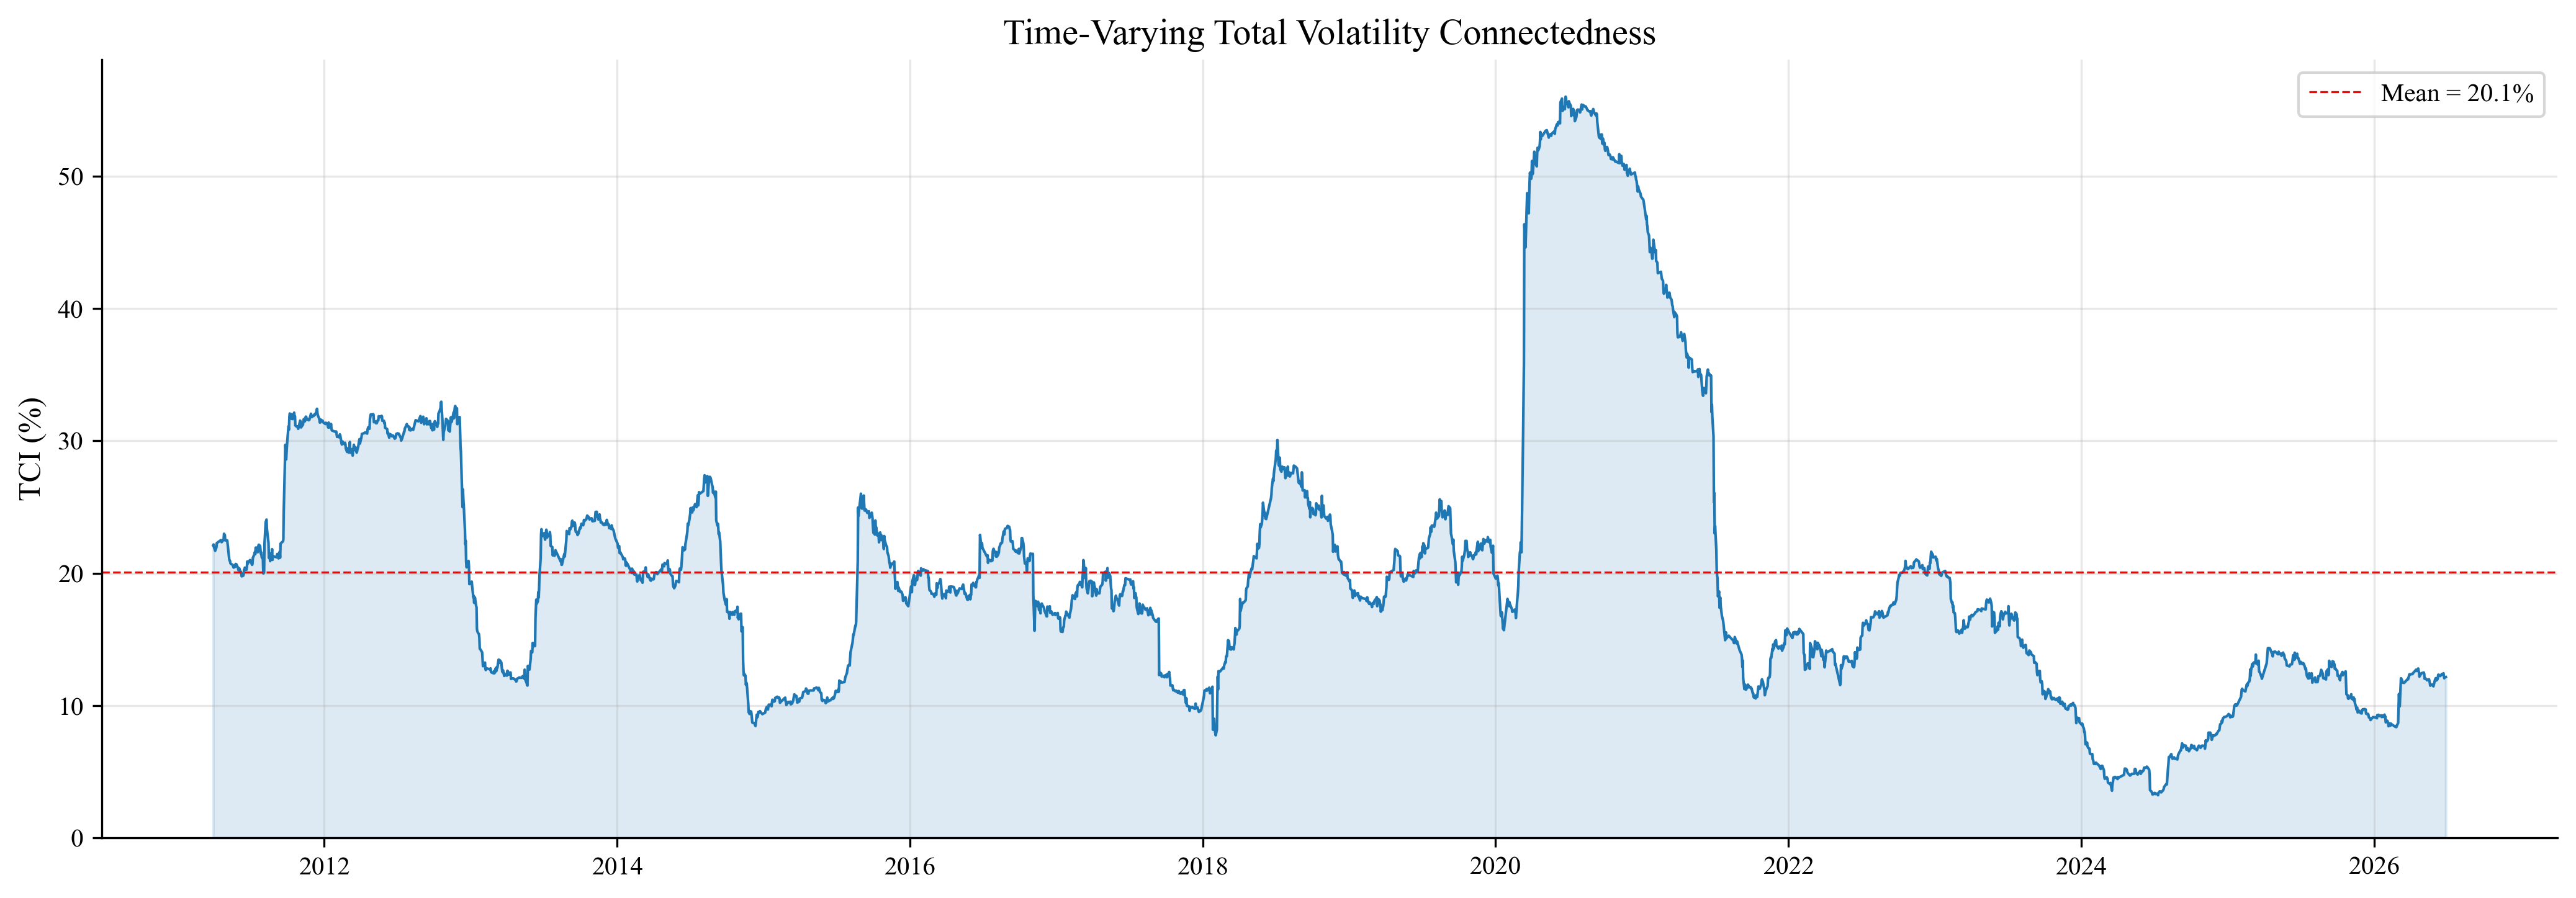
\includegraphics[width=0.98\textwidth]{../outputs/figures/tci_rolling_vol_parkinson_intersection.png}
\caption{Time-varying total volatility connectedness among ASEAN equity markets}
\label{fig:tci}
\begin{minipage}{0.90\textwidth}
\footnotesize\textit{Note:} The TCI is estimated using a 250-observation rolling VAR and a 10-day forecast horizon. The dashed line marks the full rolling-sample mean.
\end{minipage}
\end{figure}

\subsection{Net transmitters and receivers}

Directional roles are also time varying. Under the baseline specification, Indonesia has the largest positive average net contribution (0.95 percentage points), while Vietnam's average is $-0.72$. Vietnam nevertheless acts as a net transmitter in 37.5\% of rolling windows. Event-specific changes are often larger than the unconditional rankings. During COVID-19, Thailand's net position rises by 17.75 points while Vietnam's falls by 12.16 points, making Thailand a substantially stronger transmitter and Vietnam a stronger receiver. During the US--China trade-war escalation, Thailand and Vietnam both move toward transmission, by 10.45 and 6.44 points, respectively. These reversals support the time-varying component of H2 but warn against treating any market's systemic role as permanent.

\begin{figure}[p]
\centering
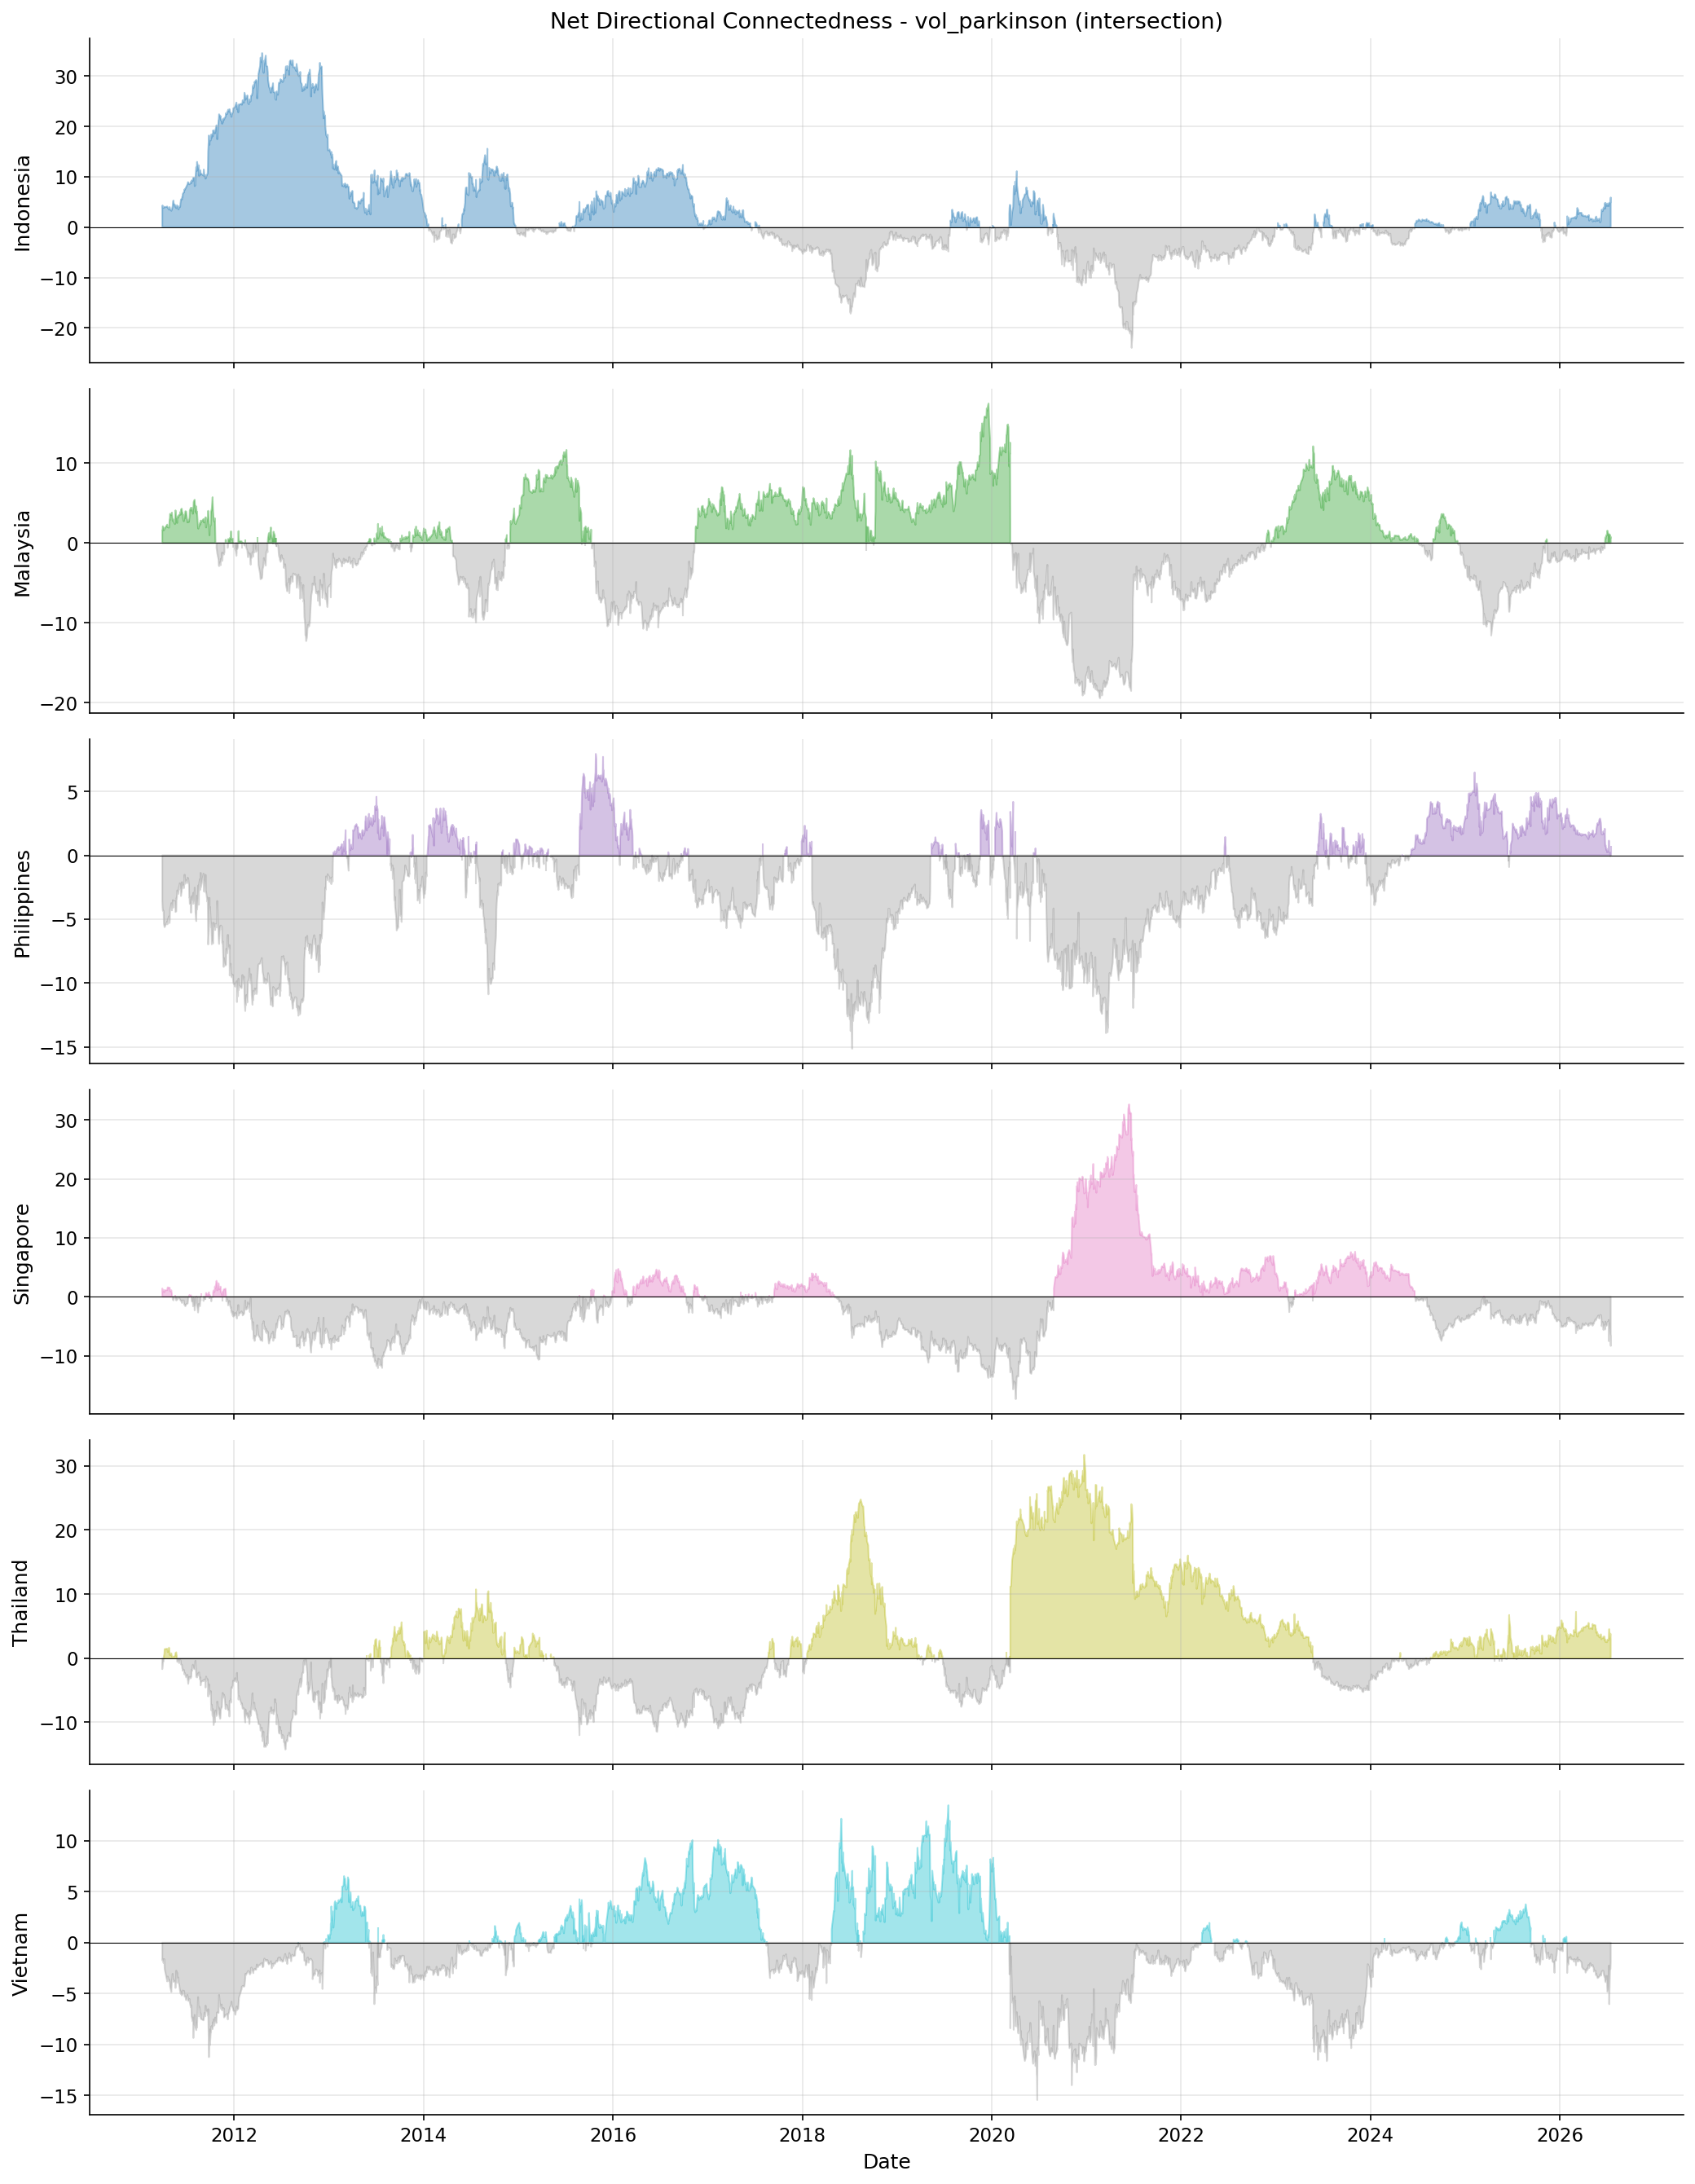
\includegraphics[width=\textwidth,height=0.82\textheight,keepaspectratio]{../outputs/figures/net_connectedness_vol_parkinson_intersection.png}
\caption{Time-varying net directional volatility connectedness by market}
\label{fig:net}
\begin{minipage}{0.88\textwidth}
\footnotesize\textit{Note:} Positive values identify net transmitters and negative values identify net receivers. Estimates use the baseline rolling specification.
\end{minipage}
\end{figure}

\begin{figure}[H]
\centering
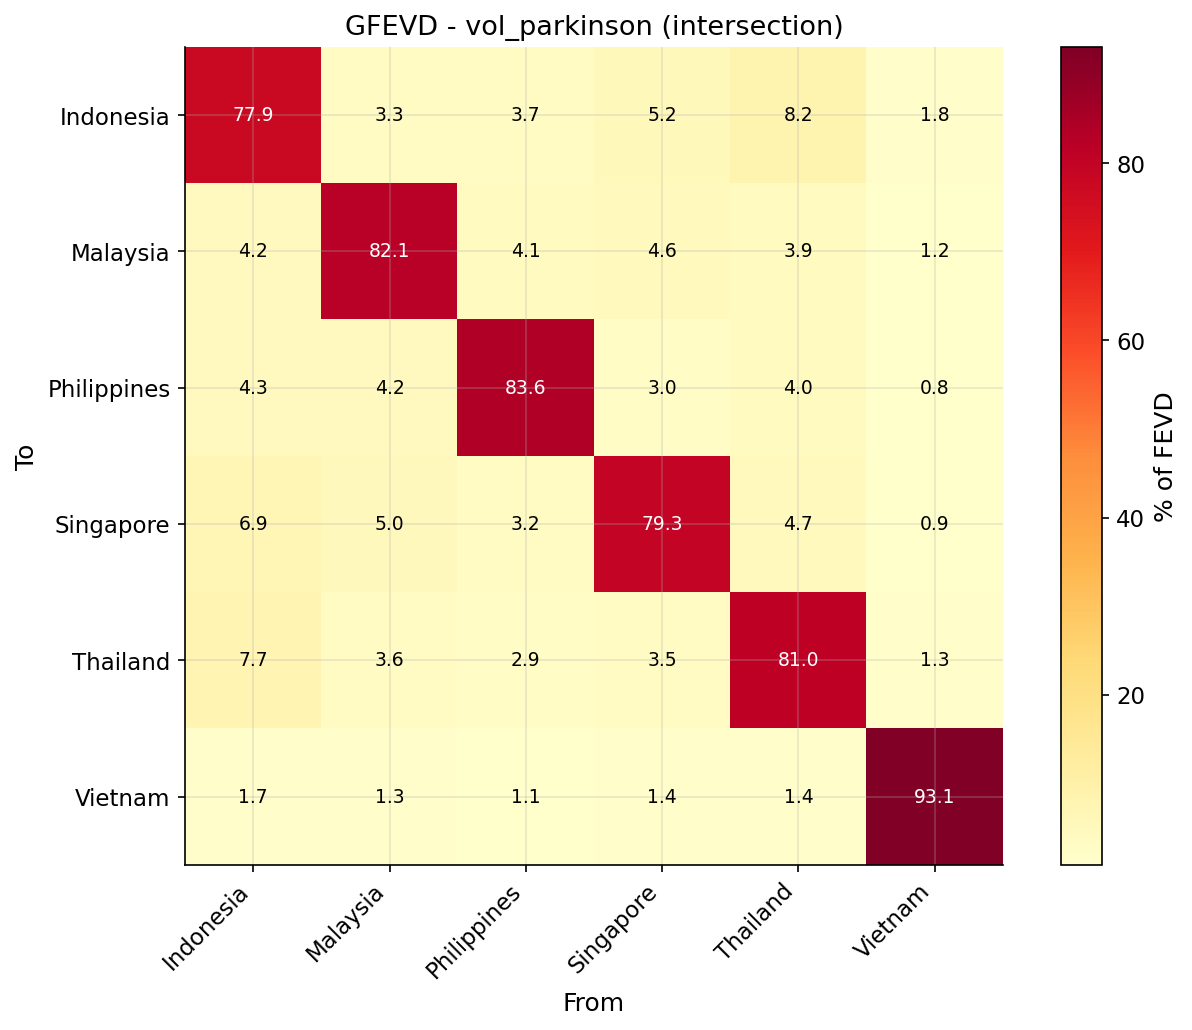
\includegraphics[width=0.74\textwidth]{../outputs/figures/gfevd_heatmap_vol_parkinson_intersection.png}
\caption{Sources and recipients of full-sample volatility transmission}
\label{fig:gfevd}
\begin{minipage}{0.88\textwidth}
\footnotesize\textit{Note:} Rows identify affected markets and columns identify shock sources. Diagonal entries are own-market variance shares; off-diagonal entries measure cross-market transmission.
\end{minipage}
\end{figure}

Figure~\ref{fig:net} visualizes the frequent changes in transmitter and receiver status, while Figure~\ref{fig:gfevd} highlights Vietnam's comparatively large own-market variance share and weak bilateral transmission.

\subsection{Global uncertainty and connectedness}

Table~\ref{tab:events} compares the rolling TCI during each shock window with its tranquil benchmark. Six of the eight episodes display a positive difference whose 20-day moving-block bootstrap interval excludes zero. The largest change occurs during COVID-19: mean connectedness rises from 21.77\% to 41.75\%, a difference of 19.98 points. The US--China trade-war escalation produces the second-largest increase (12.13 points), followed by the Chinese market crash (8.53 points), European debt crisis (7.63 points), taper tantrum (7.24 points), and 2022 monetary tightening (4.69 points). The Russia--Ukraine window produces a small and statistically uncertain increase of 0.61 points. Connectedness falls by 2.16 points during the 2023 US banking crisis. Crucially, after adjusting for multiple testing across all eight events using Holm--Bonferroni FWER and Benjamini--Hochberg FDR corrections, all six identified increases remain statistically significant at the 5\% level ($p_{\text{Holm}} < 0.01$). H1 is therefore partially, rather than universally, supported.

\begin{table}[H]
\centering
\caption{Shock-associated changes in total connectedness}
\label{tab:events}
\resizebox{\textwidth}{!}{%
\begin{tabular}{lrrrrrrl}
\toprule
Episode & Shock TCI & Tranquil TCI & Difference & 95\% MBB interval & Raw $p$ & Holm $p$ & Shift? \\
\midrule
European debt crisis & 28.73 & 21.10 & 7.63 & [5.53, 10.09] & $<0.001$ & $<0.001$ & Yes \\
Taper tantrum & 20.75 & 13.51 & 7.24 & [5.80, 10.04] & $<0.001$ & $<0.001$ & Yes \\
China market crash & 18.82 & 10.29 & 8.53 & [6.04, 11.60] & $<0.001$ & $<0.001$ & Yes \\
US--China trade war & 23.86 & 11.73 & 12.13 & [11.08, 15.46] & $<0.001$ & $<0.001$ & Yes \\
COVID-19 pandemic & 41.75 & 21.77 & 19.98 & [7.56, 31.12] & 0.001 & 0.004 & Yes \\
Russia--Ukraine war & 13.82 & 13.21 & 0.61 & [-0.92, 2.08] & 0.237 & 0.237 & No \\
Monetary tightening & 17.90 & 13.21 & 4.69 & [2.57, 7.04] & $<0.001$ & $<0.001$ & Yes \\
US banking crisis & 16.87 & 19.03 & -2.16 & [-3.75, -0.72] & 0.002 & 0.004 & No \\
\bottomrule
\end{tabular}}
\begin{minipage}{0.92\textwidth}
\footnotesize\textit{Note:} MBB denotes a moving-block bootstrap with a 20-trading-day block ($B=20$). Raw $p$ values and Holm--Bonferroni family-wise error-corrected $p$ values (as well as Benjamini--Hochberg FDR $p$ values) confirm that the six shock-associated increases remain statistically significant at the 5\% level after adjusting for multiple testing across all eight events.
\end{minipage}
\end{table}

Table~\ref{tab:hac} reports the monthly regression results. A one-point increase in average VIX is associated with a 0.96-point increase in ASEAN connectedness, holding the other variables constant. Monthly oil-price growth is also positively associated with connectedness. In contrast, the GPR coefficient is negative and statistically significant. This result is consistent with temporary regional decoupling during some geopolitical episodes, but the regression cannot identify that mechanism directly. Standardized beta coefficients confirm that VIX ($\beta^* = 0.557$) and GPR ($\beta^* = -0.467$) dominate economic magnitude. Robustness regressions using lagged uncertainty ($\text{VIX}_{m-1}$ and $\text{GPR}_{m-1}$), log-transformed GPR ($\ln\text{GPR}$), and GPR threat vs. act decompositions yield consistent findings (supplementary output \texttt{hac\_regression\_robustness.csv}). Dollar appreciation, S\&P 500 returns, and changes in the two-year Treasury yield are statistically insignificant. The model explains 48.1\% of monthly variation in the TCI and is jointly significant. H4 consequently receives mixed support: market-based uncertainty measured by VIX strengthens connectedness, whereas geopolitical risk does not have the hypothesized positive conditional association.

\begin{table}[H]
\centering
\caption{Global conditions and ASEAN total connectedness}
\label{tab:hac}
\begin{tabular}{lrrrr}
\toprule
Variable & Coefficient & HAC std. error & $t$ statistic & $p$ value \\
\midrule
Intercept & 16.379 & 3.132 & 5.229 & $<0.001$ \\
VIX & 0.962 & 0.258 & 3.724 & $<0.001$ \\
GPR & -0.130 & 0.029 & -4.438 & $<0.001$ \\
$\Delta$Oil & 0.120 & 0.056 & 2.153 & 0.031 \\
$\Delta$Dollar & -0.367 & 0.506 & -0.726 & 0.468 \\
$\Delta$S\&P 500 & 0.249 & 0.153 & 1.627 & 0.104 \\
$\Delta$US two-year yield & 2.263 & 2.888 & 0.784 & 0.433 \\
\midrule
Observations & \multicolumn{4}{r}{185} \\
$R^2$ / adjusted $R^2$ & \multicolumn{4}{r}{0.481 / 0.464} \\
HAC maximum lag & \multicolumn{4}{r}{12 months} \\
$F$ statistic ($p$ value) & \multicolumn{4}{r}{5.929 ($<0.001$)} \\
\bottomrule
\end{tabular}
\begin{minipage}{0.90\textwidth}
\footnotesize\textit{Note:} The dependent variable is the month-end rolling TCI. VIX and GPR are monthly averages. Oil, dollar, and S\&P 500 variables are monthly percentage changes; the Treasury yield is a monthly percentage-point change. Standard errors are Newey--West HAC estimates.
\end{minipage}
\end{table}

\subsection{Comparison with prior ASEAN evidence}

The findings reinforce, but also qualify, earlier evidence on ASEAN volatility transmission. The sharp increases in regional connectedness during COVID-19, the US--China trade-war escalation, and the taper tantrum are consistent with \citet{VoTran2020}, who show that shocks from the US equity market spill over to ASEAN markets, and with \citet{Chow2017}, who links Asian-market exposure to financial openness. The COVID-19 increase also accords with \citet{SethapramoteEtAl2023}, who find stronger global-to-ASEAN and intraregional spillovers during the pandemic. The present estimates extend those studies by identifying how a common external disturbance is redistributed \emph{within} the ASEAN network across several episodes: Indonesia and Thailand are the principal full-sample transmitters, whereas Singapore is a net receiver in the baseline model.

The results for Vietnam add a further qualification. \citet{VoEllis2018} document Vietnam's increasing linkages with advanced markets, while \citet{AlAnshari2025} find relatively weak full-period correlations between Vietnam and the other ASEAN-6 markets but identify Vietnam as informative for distinguishing network regimes. The large own-market variance share found here is consistent with that relative separation, yet the directional estimates show that separation is not equivalent to a permanently passive role. Vietnam is a modest receiver under the range-based baseline but becomes a transmitter under some return-based proxies. This measurement sensitivity complements the policy-uncertainty evidence of \citet{HoqueEtAl2026}: the direction and strength of ASEAN connectedness depend on both the source of uncertainty and the empirical representation of volatility. Accordingly, the contribution of this study is not a universal ranking of markets, but evidence that regional systemic roles are state and measurement dependent.

\section{Robustness and Additional Analysis}
\label{sec:robustness}

The aggregate finding of positive, time-varying ASEAN connectedness survives changes in the forecast horizon, rolling-window length, currency denomination, frequency, and VAR lag order. Figure~\ref{fig:robustness-comparison} summarizes the sensitivity of mean TCI to the volatility proxy, sampling frequency, rolling-window length, and forecast horizon, while Table~\ref{tab:robustness} reports representative specifications and Vietnam's directional position. To address information-criterion selections and residual autocorrelation diagnostics (where BIC selects lag 1 or 3, HQIC selects lag 4, and AIC selects lag 7), we estimate fixed VAR lag orders $p \in \{1, 2, 3, 4, 7\}$. Across these orders, mean TCI values are 20.04\% ($p=1$), 20.85\% ($p=2$), 21.62\% ($p=3$), 22.06\% ($p=4$, HQIC), and 24.76\% ($p=7$, AIC), demonstrating that total connectedness remains stable within 20\%--25\% and Vietnam consistently maintains a modest net receiver role ($\text{Net}_{\text{Vietnam}} < 0$).

The magnitude of connectedness is nevertheless sensitive to the volatility proxy and sampling frequency. Panel~1 shows that weekly estimates exceed their daily counterparts for all five proxies, with the largest frequency difference under the Parkinson measure. Panels~2 and 3 show that the daily mean TCI is comparatively stable across rolling windows of 200, 250, and 300 trading days and forecast horizons of 5, 10, and 20 days; the ordering across proxies is also preserved. More importantly for H3, Vietnam is a net receiver in the Parkinson and US-dollar specifications but a net transmitter in local-currency squared- and absolute-return specifications. Its share of net-transmitter windows ranges from approximately 37\% to 67\%. The hypothesis that Vietnam is generally a receiver is therefore supported by the baseline range-based model but not robust across all measurement choices. A return-based GARCH-filtered EWMA exercise is retained as supplementary correlation evidence and is not presented as a DCC-GARCH model.

\clearpage
\begin{landscape}
\begin{figure}[p]
\centering
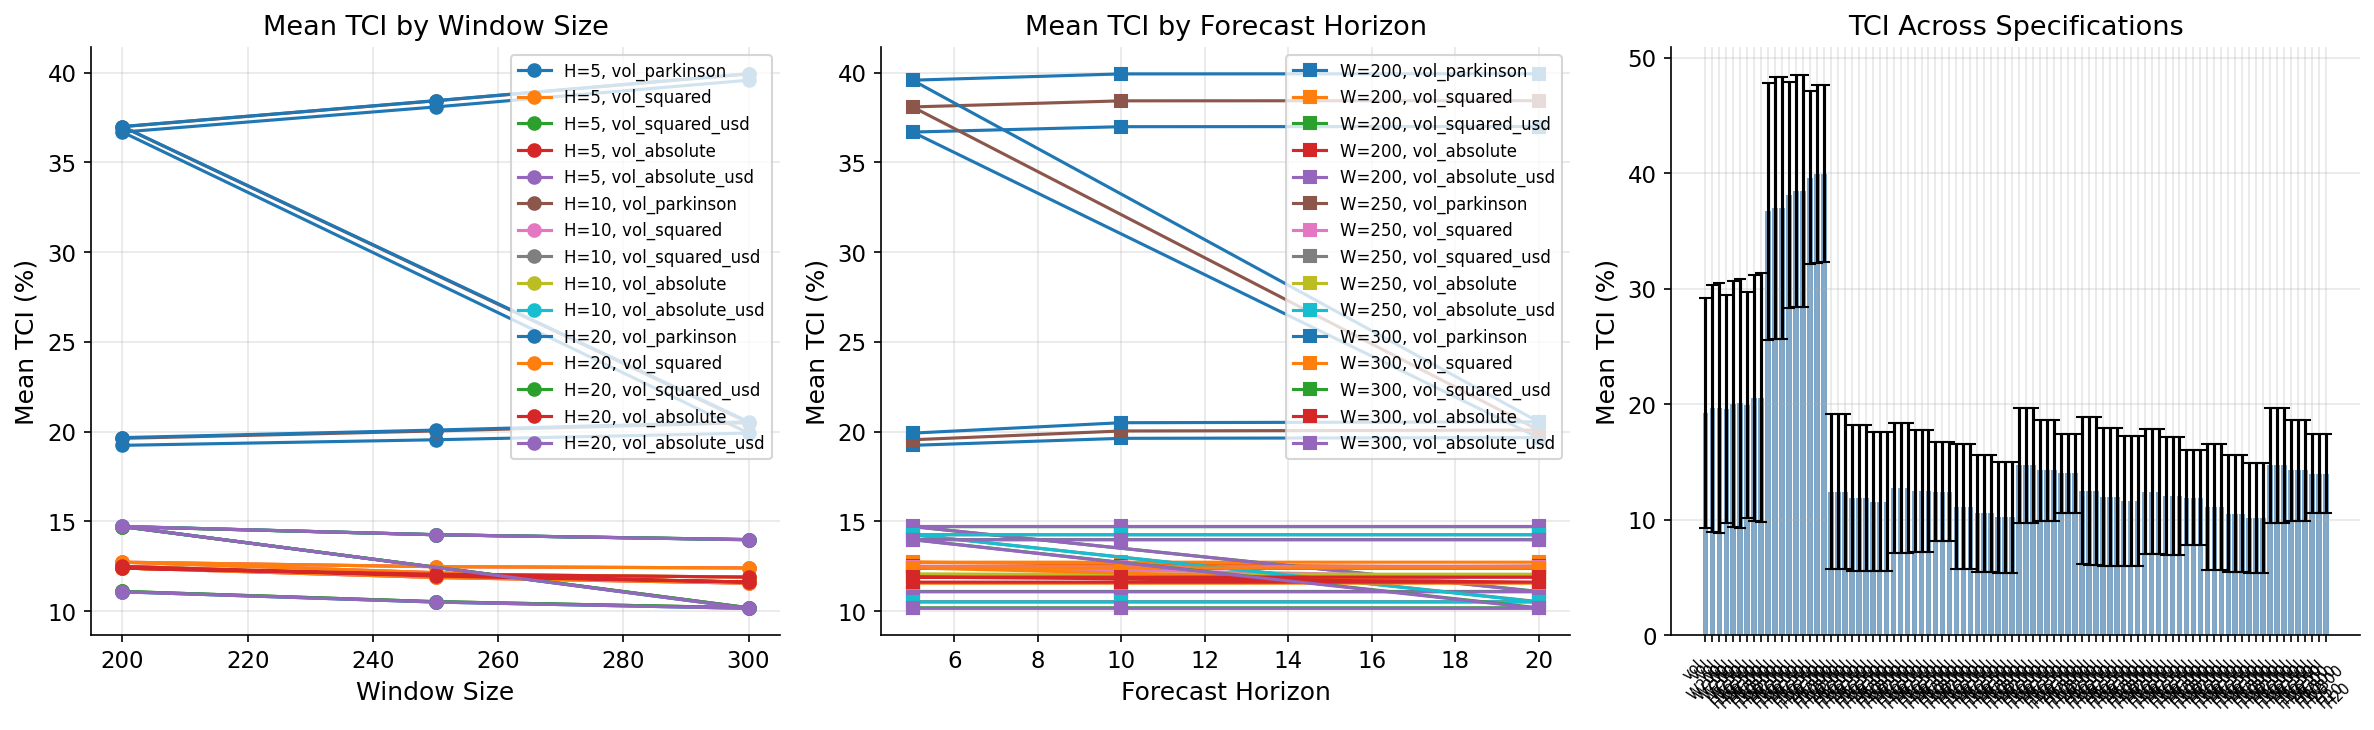
\includegraphics[width=0.98\linewidth]{../outputs/figures/robustness_comparison.png}
\caption{Robustness of mean total connectedness}
\label{fig:robustness-comparison}
\begin{minipage}{0.96\linewidth}
\footnotesize\textit{Note:} Panel~1 compares daily and weekly mean TCI estimates across the Parkinson, squared-return, US-dollar squared-return, absolute-return, and US-dollar absolute-return volatility proxies; error bars denote standard errors. Panel~2 reports daily mean TCI for rolling-window lengths $W\in\{200,250,300\}$ trading days. Panel~3 reports daily mean TCI for forecast horizons $H\in\{5,10,20\}$ days. In Panels~2 and 3, the non-varied baseline settings are $W=250$ and $H=10$.
\end{minipage}
\end{figure}
\end{landscape}
\clearpage

\begin{table}[H]
\centering
\caption{Selected robustness results}
\label{tab:robustness}
\resizebox{\textwidth}{!}{%
\begin{tabular}{llrrr}
\toprule
Frequency/proxy & Currency/specification & Mean TCI & Mean net VNM & VNM transmitter (\%) \\
\midrule
Daily Parkinson & 250 days, $H=10$ (Baseline) & 20.04 & -0.72 & 37.52 \\
Daily Parkinson & 200 days, $H=10$ & 19.63 & -1.05 & 41.63 \\
Daily Parkinson & 300 days, $H=10$ & 20.50 & -0.51 & 37.09 \\
Daily squared return & Local currency & 11.88 & 0.64 & 64.07 \\
Daily squared return & US dollar & 10.53 & -0.20 & 40.60 \\
Daily absolute return & Local currency & 11.96 & 0.66 & 67.34 \\
Daily absolute return & US dollar & 10.51 & -0.17 & 40.69 \\
Weekly Parkinson & 50 weeks, $H=2$ & 33.86 & -2.00 & 38.79 \\
Weekly Parkinson & 40 weeks, $H=2$ & 35.14 & -1.91 & 39.80 \\
\bottomrule
\end{tabular}}
\begin{minipage}{0.92\textwidth}
\footnotesize\textit{Note:} Mean net VNM is Vietnam's average TO-minus-FROM connectedness. Positive values indicate a net transmitter. All figures are synchronized with the authoritative \texttt{manuscript\_results.json} dataset. The empirical mean TCI for daily log squared returns ($W=250, H=10$) is validated at 11.88\%.
\end{minipage}
\end{table}

\section{Conclusions and Policy Implications}
\label{sec:conclusion}

This paper examines volatility transmission among six ASEAN equity markets from January 2010 to July 2026. The full-sample TCI of approximately 17.15\% confirms economically meaningful regional interdependence, while the rolling mean of 20.04\% and maximum of 48.84\% show that the intensity of transmission varies markedly over time. Thailand and Indonesia are net transmitters in the full-sample baseline, and Vietnam has the largest own-market variance share and a modest net-receiver position.

The event evidence shows that global disturbances do not affect the ASEAN network uniformly. Six of eight episodes are associated with significant increases in connectedness, and the COVID-19 period produces by far the largest change. Russia's invasion of Ukraine does not generate a statistically distinguishable increase within the selected window, while connectedness declines during the US banking crisis. Likewise, the continuous-indicator regression finds a positive association with VIX and oil-price changes but a negative association with geopolitical risk. These differences caution against treating all forms of global uncertainty as equivalent.

For investors, the results imply that regional diversification benefits are state dependent and can deteriorate during periods of market-wide stress. For policymakers, monitoring directional measures is useful because the markets transmitting risk can change across episodes. The sensitivity of Vietnam's net position is itself an important finding: its classification depends on the volatility proxy, currency denomination, and frequency, even though the baseline model identifies it as relatively insulated and usually a receiver.

Several limitations qualify the conclusions. Rolling estimates overlap mechanically, event windows cannot fully isolate concurrent shocks, and the uncertainty regressions establish association rather than causality. Range-based, squared-return, and absolute-return volatility measures capture different features of market variation, producing differences in estimated connectedness. Future research could apply a time-varying-parameter VAR, examine tail or frequency-specific connectedness, or extend the network to ASEAN exchange rates and sectoral equity indices.

\section*{Declarations}

\textbf{Funding:} This research received no external funding.

\textbf{Conflicts of interest:} The authors declare no conflicts of interest.

\textbf{Data availability:} The study uses market data from Yahoo Finance and VNStock and global variables from Federal Reserve Economic Data and the Caldara--Iacoviello Geopolitical Risk Index. Processed data, event-window definitions, and derived results are available in the \href{https://github.com/DeckardShaw31/Time-Varying-Volatility-Connectedness-among-ASEAN-Equity-Markets}{project repository}.

\textbf{Code availability:} Replication code and documented outputs are available in the \href{https://github.com/DeckardShaw31/Time-Varying-Volatility-Connectedness-among-ASEAN-Equity-Markets}{project repository}.

\appendix
\section*{Appendix A: Supplementary Time-Series Figures}
\label{app:diagnostic-figures}
\renewcommand{\thefigure}{A\arabic{figure}}
\setcounter{figure}{0}

\begin{center}
\centering
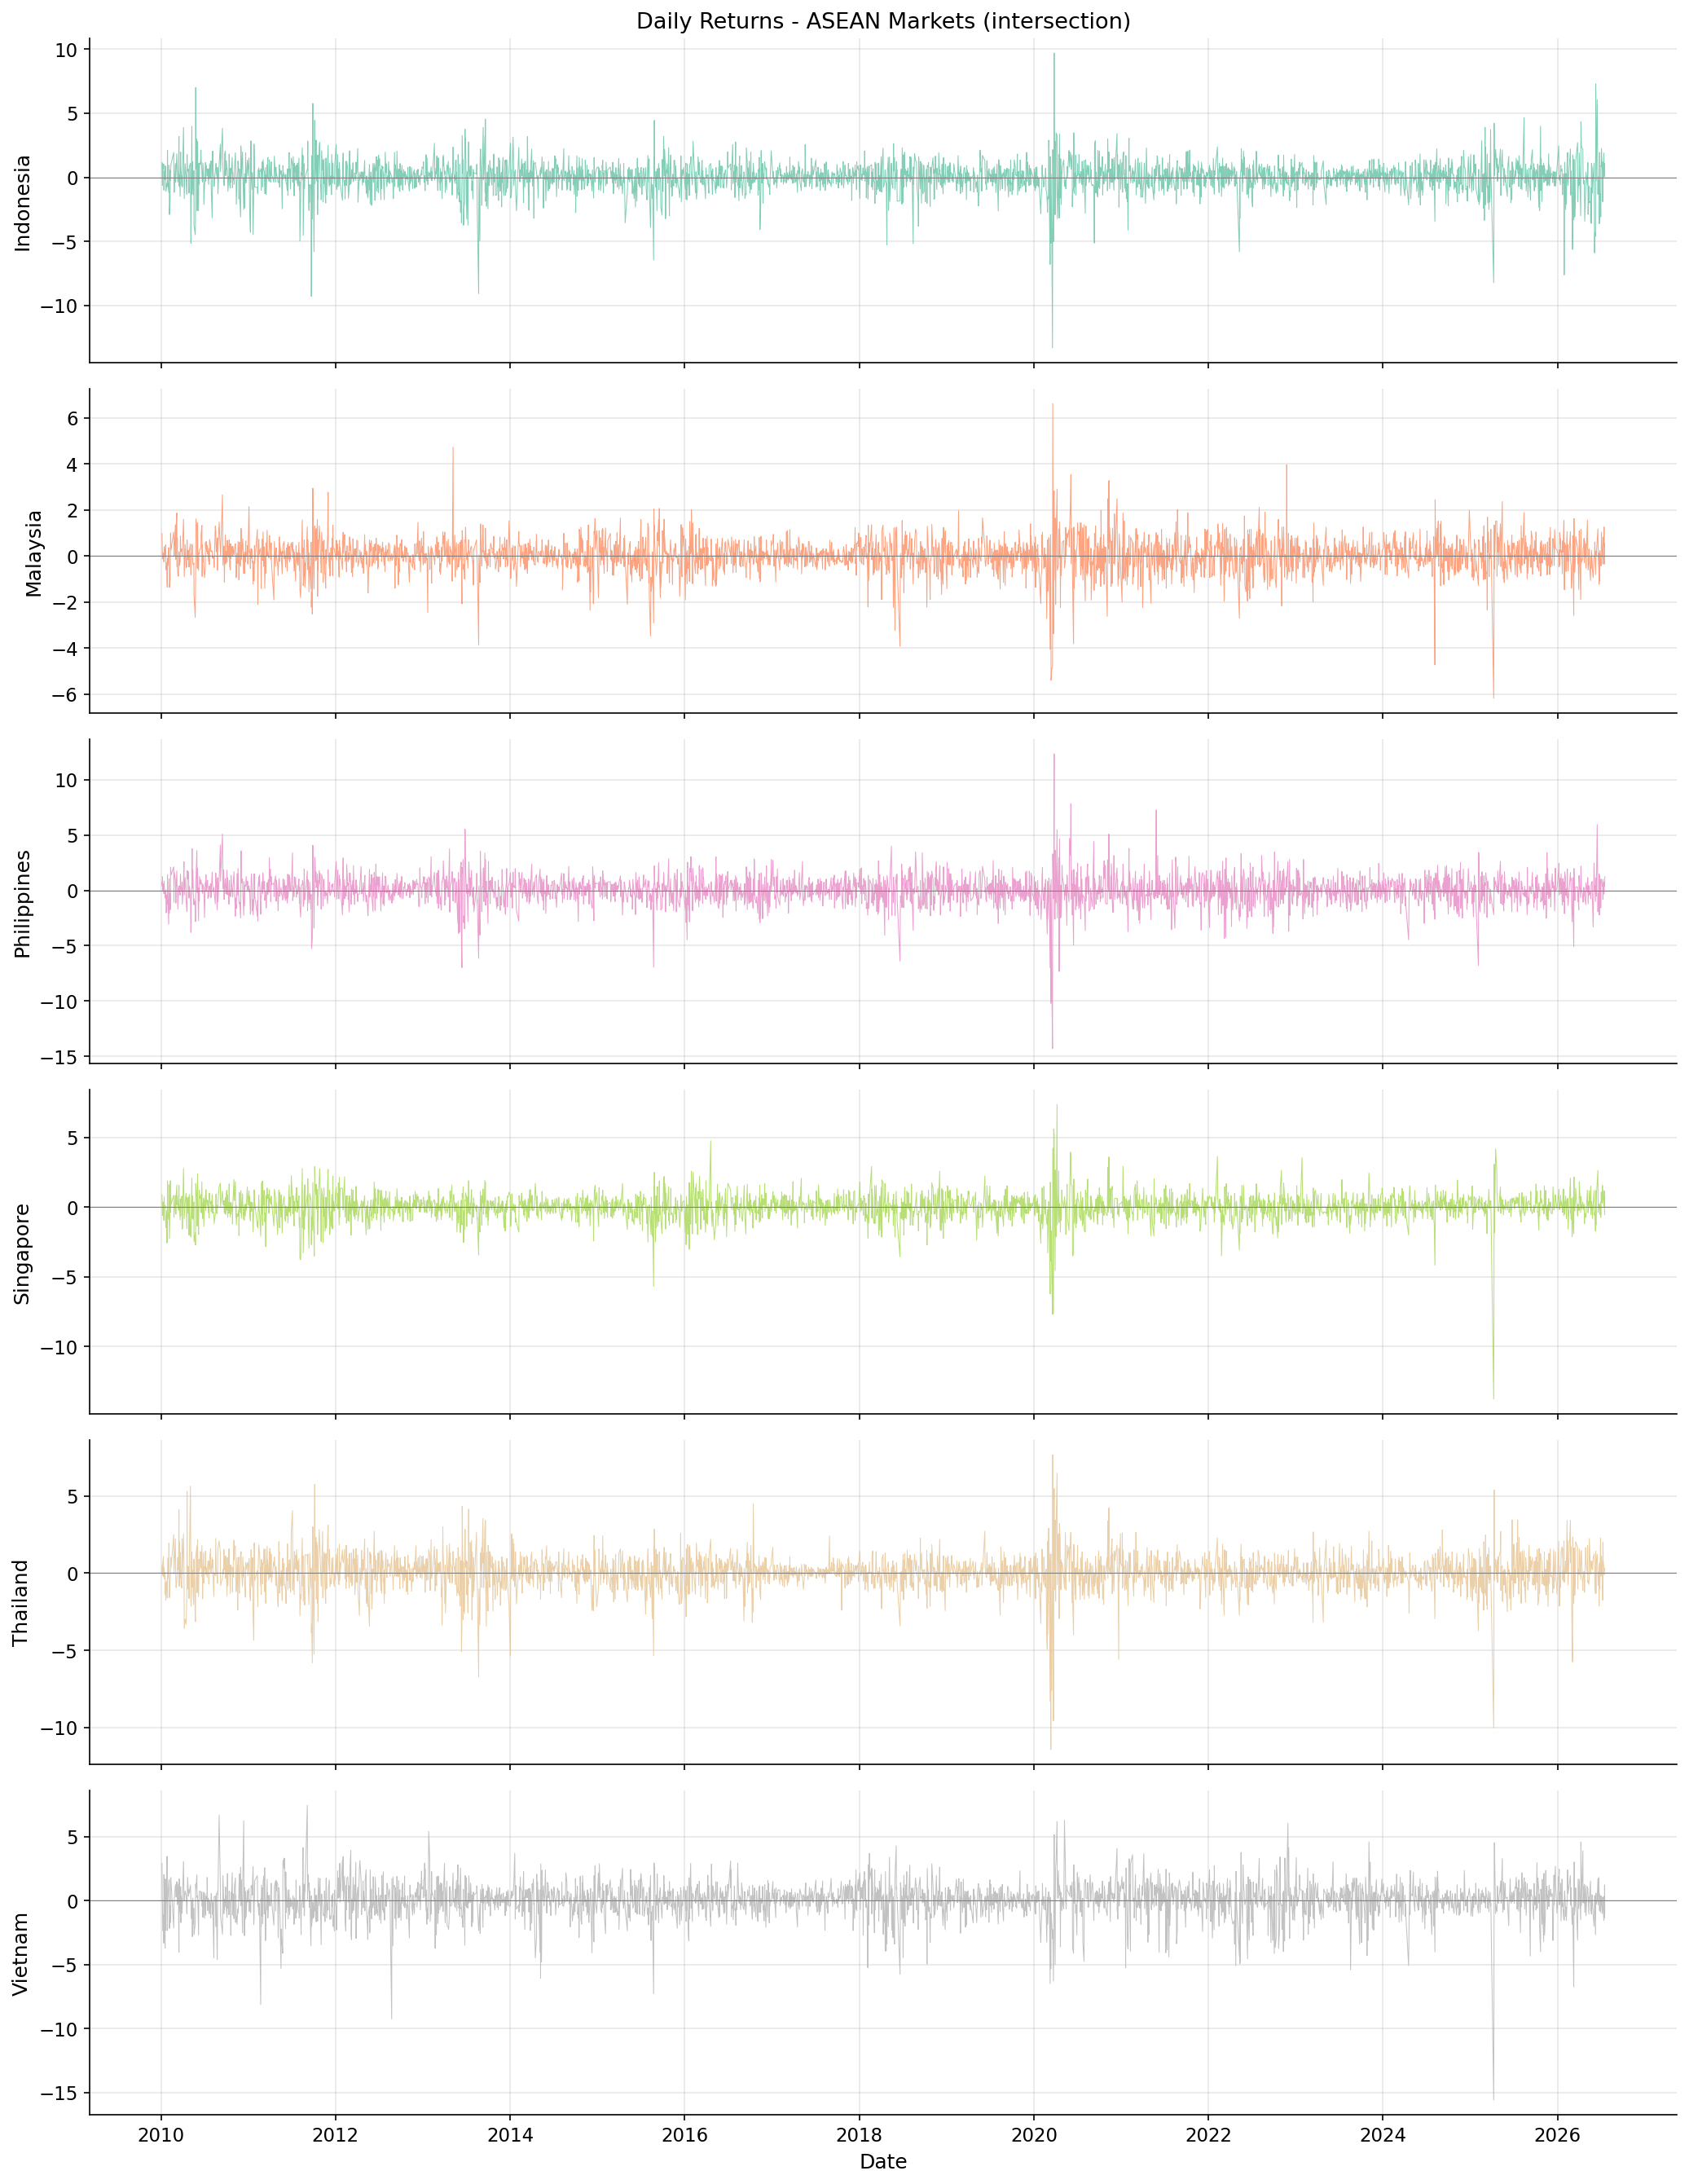
\includegraphics[width=0.78\textwidth,trim=0 643bp 0 0,clip]{../outputs/figures/returns_timeseries_intersection.png}
\captionof{figure}{Daily local-currency equity-index returns: Indonesia, Malaysia, and the Philippines}
\label{fig:returns-top}
\begin{minipage}{0.78\textwidth}
\small\textit{Note:} Returns are continuously compounded percentages calculated on trading dates common to all six markets.
\end{minipage}
\end{center}

\begin{center}
\centering
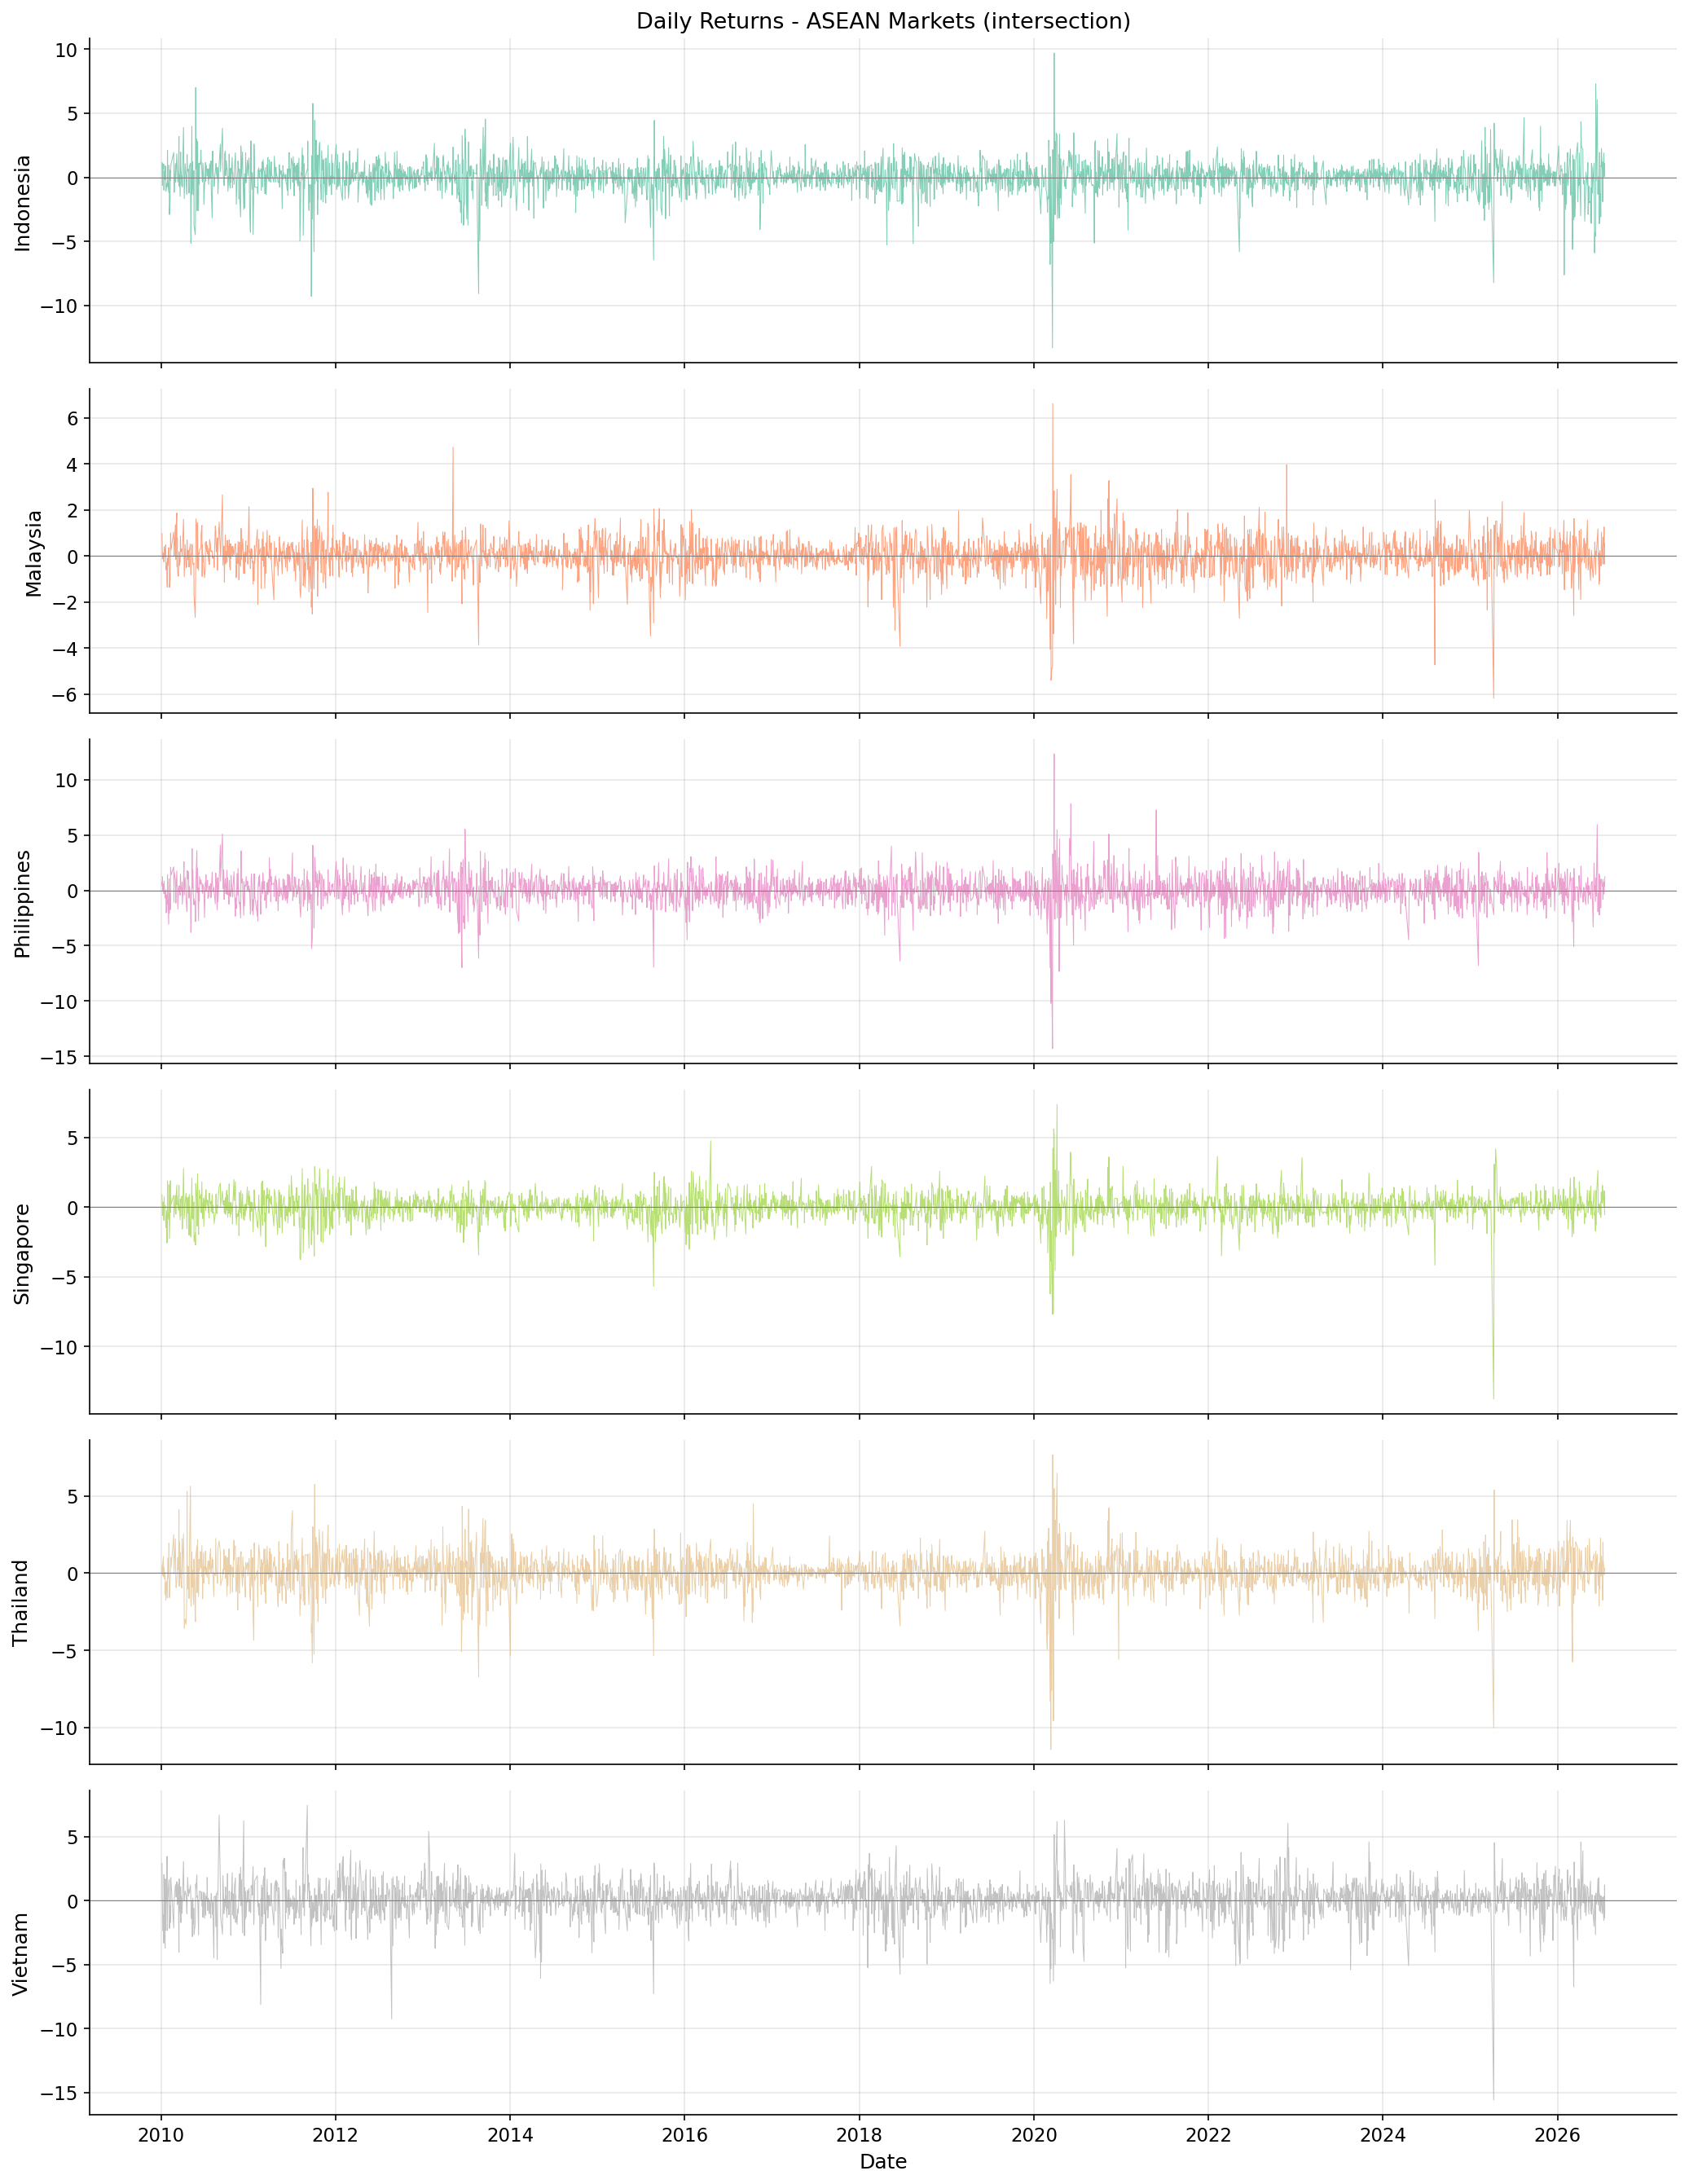
\includegraphics[width=0.78\textwidth,trim=0 0 0 643bp,clip]{../outputs/figures/returns_timeseries_intersection.png}
\captionof{figure}{Daily local-currency equity-index returns: Singapore, Thailand, and Vietnam}
\label{fig:returns-bottom}
\end{center}

\clearpage
\begin{center}
\centering
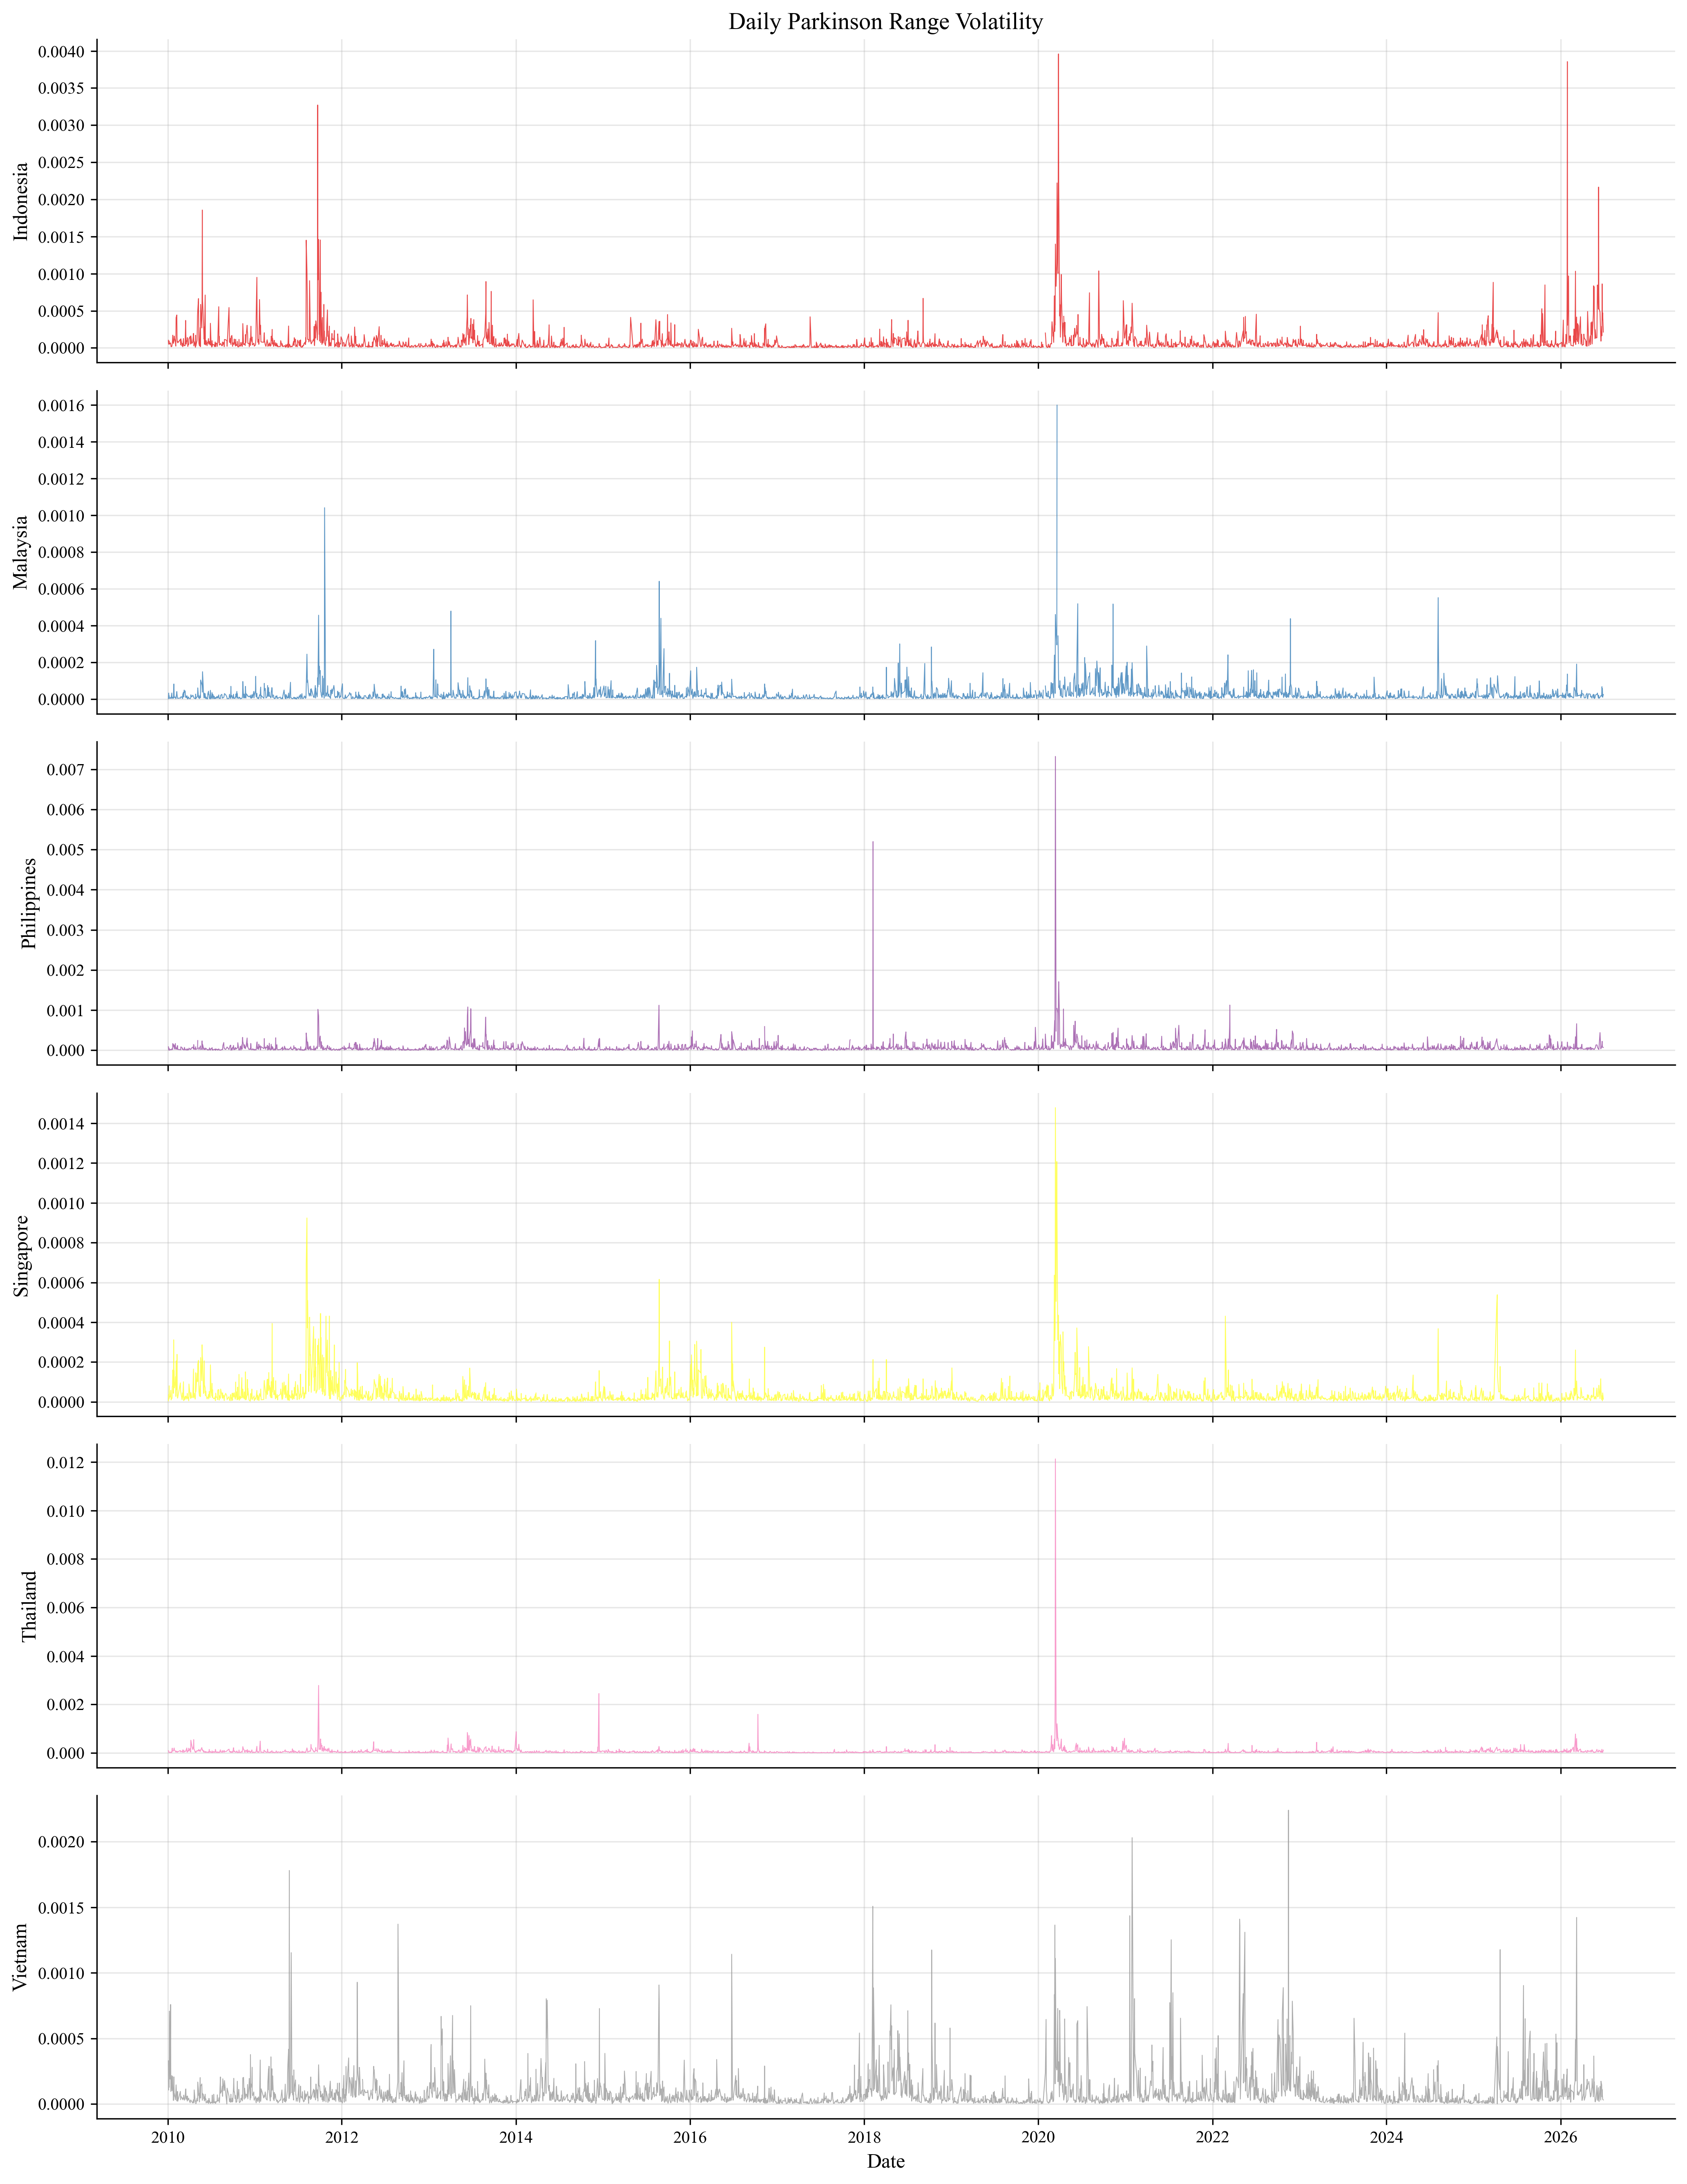
\includegraphics[width=0.78\textwidth,trim=0 643bp 0 0,clip]{../outputs/figures/volatility_vol_parkinson_intersection.png}
\captionof{figure}{Daily Parkinson range-volatility estimates: Indonesia, Malaysia, and the Philippines}
\label{fig:volatility-top}
\begin{minipage}{0.78\textwidth}
\small\textit{Note:} The figure presents unlogged Parkinson estimates. The connectedness model uses the logarithmic transformation of each series.
\end{minipage}
\end{center}

\begin{center}
\centering
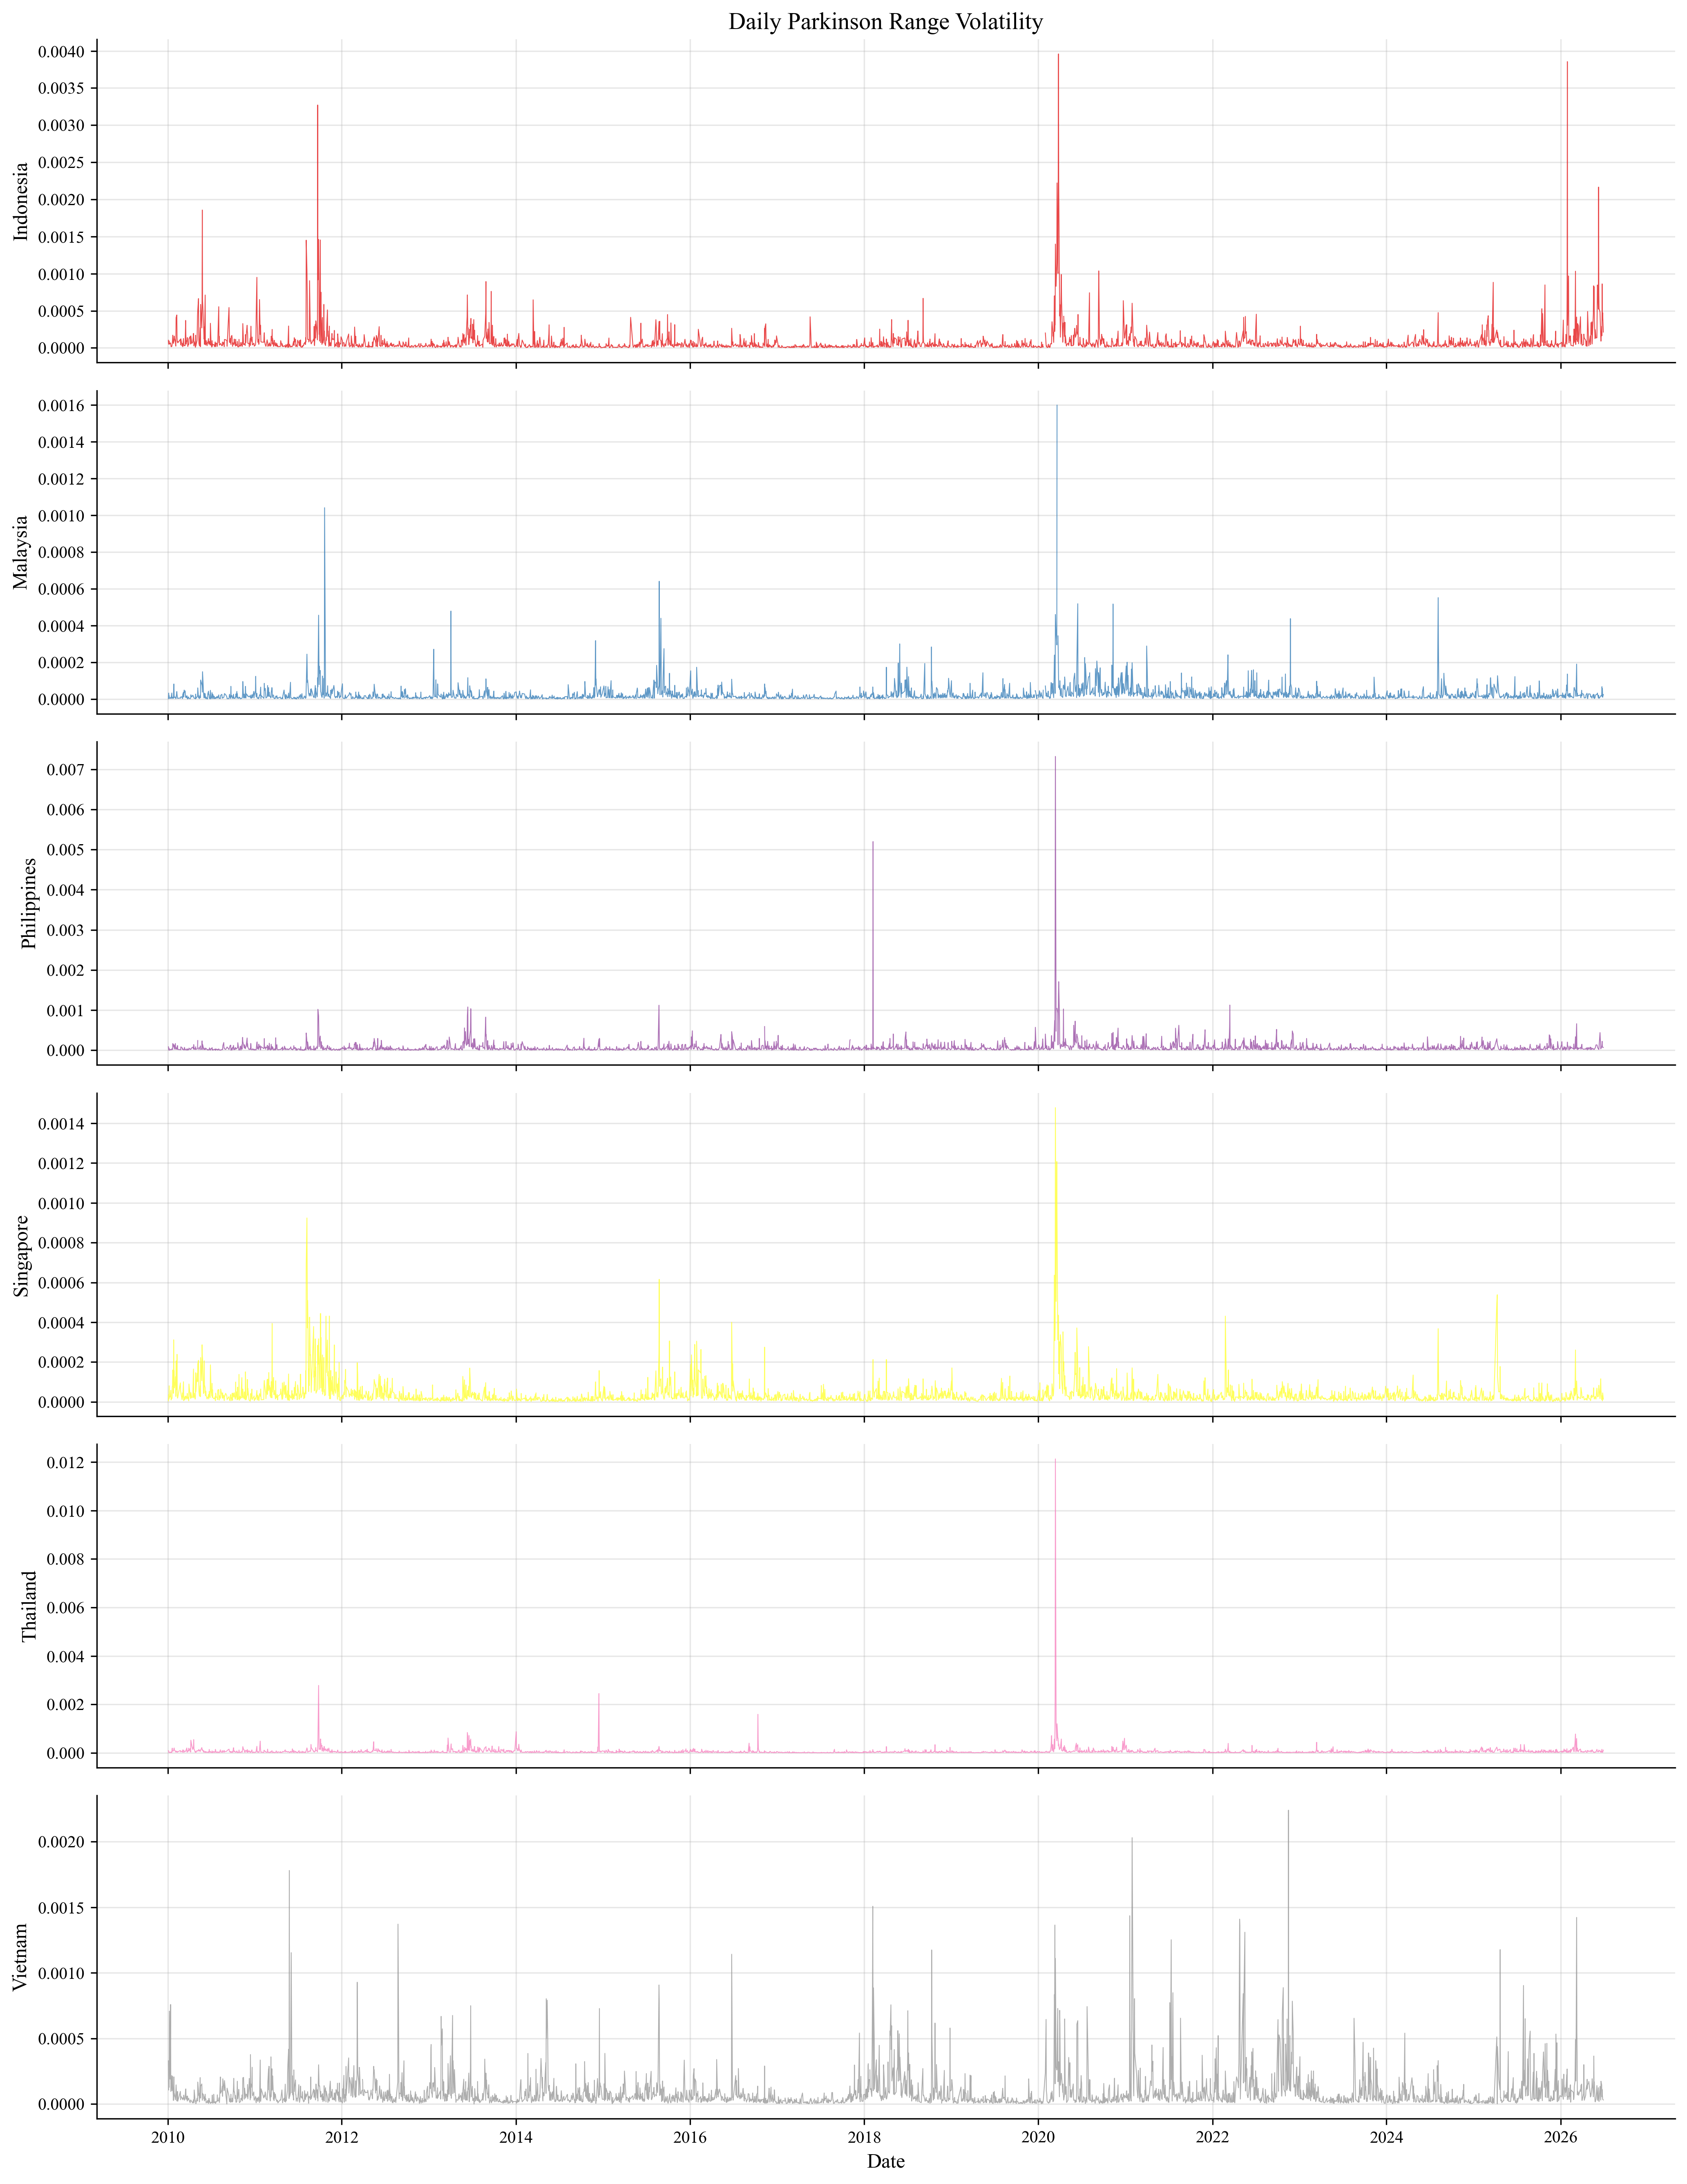
\includegraphics[width=0.78\textwidth,trim=0 0 0 643bp,clip]{../outputs/figures/volatility_vol_parkinson_intersection.png}
\captionof{figure}{Daily Parkinson range-volatility estimates: Singapore, Thailand, and Vietnam}
\label{fig:volatility-bottom}
\end{center}

\bibliographystyle{plainnat}
\bibliography{references}

\end{document}
